% Options for packages loaded elsewhere
% Options for packages loaded elsewhere
\PassOptionsToPackage{unicode}{hyperref}
\PassOptionsToPackage{hyphens}{url}
\PassOptionsToPackage{dvipsnames,svgnames,x11names}{xcolor}
%
\documentclass[
  letterpaper,
  DIV=11,
  numbers=noendperiod]{scrartcl}
\usepackage{xcolor}
\usepackage{amsmath,amssymb}
\setcounter{secnumdepth}{-\maxdimen} % remove section numbering
\usepackage{iftex}
\ifPDFTeX
  \usepackage[T1]{fontenc}
  \usepackage[utf8]{inputenc}
  \usepackage{textcomp} % provide euro and other symbols
\else % if luatex or xetex
  \usepackage{unicode-math} % this also loads fontspec
  \defaultfontfeatures{Scale=MatchLowercase}
  \defaultfontfeatures[\rmfamily]{Ligatures=TeX,Scale=1}
\fi
\usepackage{lmodern}
\ifPDFTeX\else
  % xetex/luatex font selection
\fi
% Use upquote if available, for straight quotes in verbatim environments
\IfFileExists{upquote.sty}{\usepackage{upquote}}{}
\IfFileExists{microtype.sty}{% use microtype if available
  \usepackage[]{microtype}
  \UseMicrotypeSet[protrusion]{basicmath} % disable protrusion for tt fonts
}{}
\makeatletter
\@ifundefined{KOMAClassName}{% if non-KOMA class
  \IfFileExists{parskip.sty}{%
    \usepackage{parskip}
  }{% else
    \setlength{\parindent}{0pt}
    \setlength{\parskip}{6pt plus 2pt minus 1pt}}
}{% if KOMA class
  \KOMAoptions{parskip=half}}
\makeatother
% Make \paragraph and \subparagraph free-standing
\makeatletter
\ifx\paragraph\undefined\else
  \let\oldparagraph\paragraph
  \renewcommand{\paragraph}{
    \@ifstar
      \xxxParagraphStar
      \xxxParagraphNoStar
  }
  \newcommand{\xxxParagraphStar}[1]{\oldparagraph*{#1}\mbox{}}
  \newcommand{\xxxParagraphNoStar}[1]{\oldparagraph{#1}\mbox{}}
\fi
\ifx\subparagraph\undefined\else
  \let\oldsubparagraph\subparagraph
  \renewcommand{\subparagraph}{
    \@ifstar
      \xxxSubParagraphStar
      \xxxSubParagraphNoStar
  }
  \newcommand{\xxxSubParagraphStar}[1]{\oldsubparagraph*{#1}\mbox{}}
  \newcommand{\xxxSubParagraphNoStar}[1]{\oldsubparagraph{#1}\mbox{}}
\fi
\makeatother


\usepackage{longtable,booktabs,array}
\usepackage{calc} % for calculating minipage widths
% Correct order of tables after \paragraph or \subparagraph
\usepackage{etoolbox}
\makeatletter
\patchcmd\longtable{\par}{\if@noskipsec\mbox{}\fi\par}{}{}
\makeatother
% Allow footnotes in longtable head/foot
\IfFileExists{footnotehyper.sty}{\usepackage{footnotehyper}}{\usepackage{footnote}}
\makesavenoteenv{longtable}
\usepackage{graphicx}
\makeatletter
\newsavebox\pandoc@box
\newcommand*\pandocbounded[1]{% scales image to fit in text height/width
  \sbox\pandoc@box{#1}%
  \Gscale@div\@tempa{\textheight}{\dimexpr\ht\pandoc@box+\dp\pandoc@box\relax}%
  \Gscale@div\@tempb{\linewidth}{\wd\pandoc@box}%
  \ifdim\@tempb\p@<\@tempa\p@\let\@tempa\@tempb\fi% select the smaller of both
  \ifdim\@tempa\p@<\p@\scalebox{\@tempa}{\usebox\pandoc@box}%
  \else\usebox{\pandoc@box}%
  \fi%
}
% Set default figure placement to htbp
\def\fps@figure{htbp}
\makeatother


% definitions for citeproc citations
\NewDocumentCommand\citeproctext{}{}
\NewDocumentCommand\citeproc{mm}{%
  \begingroup\def\citeproctext{#2}\cite{#1}\endgroup}
\makeatletter
 % allow citations to break across lines
 \let\@cite@ofmt\@firstofone
 % avoid brackets around text for \cite:
 \def\@biblabel#1{}
 \def\@cite#1#2{{#1\if@tempswa , #2\fi}}
\makeatother
\newlength{\cslhangindent}
\setlength{\cslhangindent}{1.5em}
\newlength{\csllabelwidth}
\setlength{\csllabelwidth}{3em}
\newenvironment{CSLReferences}[2] % #1 hanging-indent, #2 entry-spacing
 {\begin{list}{}{%
  \setlength{\itemindent}{0pt}
  \setlength{\leftmargin}{0pt}
  \setlength{\parsep}{0pt}
  % turn on hanging indent if param 1 is 1
  \ifodd #1
   \setlength{\leftmargin}{\cslhangindent}
   \setlength{\itemindent}{-1\cslhangindent}
  \fi
  % set entry spacing
  \setlength{\itemsep}{#2\baselineskip}}}
 {\end{list}}
\usepackage{calc}
\newcommand{\CSLBlock}[1]{\hfill\break\parbox[t]{\linewidth}{\strut\ignorespaces#1\strut}}
\newcommand{\CSLLeftMargin}[1]{\parbox[t]{\csllabelwidth}{\strut#1\strut}}
\newcommand{\CSLRightInline}[1]{\parbox[t]{\linewidth - \csllabelwidth}{\strut#1\strut}}
\newcommand{\CSLIndent}[1]{\hspace{\cslhangindent}#1}



\setlength{\emergencystretch}{3em} % prevent overfull lines

\providecommand{\tightlist}{%
  \setlength{\itemsep}{0pt}\setlength{\parskip}{0pt}}



 


\KOMAoption{captions}{tableheading}
\makeatletter
\@ifpackageloaded{tcolorbox}{}{\usepackage[skins,breakable]{tcolorbox}}
\@ifpackageloaded{fontawesome5}{}{\usepackage{fontawesome5}}
\definecolor{quarto-callout-color}{HTML}{909090}
\definecolor{quarto-callout-note-color}{HTML}{0758E5}
\definecolor{quarto-callout-important-color}{HTML}{CC1914}
\definecolor{quarto-callout-warning-color}{HTML}{EB9113}
\definecolor{quarto-callout-tip-color}{HTML}{00A047}
\definecolor{quarto-callout-caution-color}{HTML}{FC5300}
\definecolor{quarto-callout-color-frame}{HTML}{acacac}
\definecolor{quarto-callout-note-color-frame}{HTML}{4582ec}
\definecolor{quarto-callout-important-color-frame}{HTML}{d9534f}
\definecolor{quarto-callout-warning-color-frame}{HTML}{f0ad4e}
\definecolor{quarto-callout-tip-color-frame}{HTML}{02b875}
\definecolor{quarto-callout-caution-color-frame}{HTML}{fd7e14}
\makeatother
\makeatletter
\@ifpackageloaded{caption}{}{\usepackage{caption}}
\AtBeginDocument{%
\ifdefined\contentsname
  \renewcommand*\contentsname{Table of contents}
\else
  \newcommand\contentsname{Table of contents}
\fi
\ifdefined\listfigurename
  \renewcommand*\listfigurename{List of Figures}
\else
  \newcommand\listfigurename{List of Figures}
\fi
\ifdefined\listtablename
  \renewcommand*\listtablename{List of Tables}
\else
  \newcommand\listtablename{List of Tables}
\fi
\ifdefined\figurename
  \renewcommand*\figurename{Figure}
\else
  \newcommand\figurename{Figure}
\fi
\ifdefined\tablename
  \renewcommand*\tablename{Table}
\else
  \newcommand\tablename{Table}
\fi
}
\@ifpackageloaded{float}{}{\usepackage{float}}
\floatstyle{ruled}
\@ifundefined{c@chapter}{\newfloat{codelisting}{h}{lop}}{\newfloat{codelisting}{h}{lop}[chapter]}
\floatname{codelisting}{Listing}
\newcommand*\listoflistings{\listof{codelisting}{List of Listings}}
\makeatother
\makeatletter
\makeatother
\makeatletter
\@ifpackageloaded{caption}{}{\usepackage{caption}}
\@ifpackageloaded{subcaption}{}{\usepackage{subcaption}}
\makeatother
\usepackage{bookmark}
\IfFileExists{xurl.sty}{\usepackage{xurl}}{} % add URL line breaks if available
\urlstyle{same}
\hypersetup{
  pdftitle={Describing the Structure of Dynamical Systems},
  pdfauthor={Cole Prather},
  colorlinks=true,
  linkcolor={blue},
  filecolor={Maroon},
  citecolor={Blue},
  urlcolor={Blue},
  pdfcreator={LaTeX via pandoc}}


\title{Describing the Structure of Dynamical Systems}
\usepackage{etoolbox}
\makeatletter
\providecommand{\subtitle}[1]{% add subtitle to \maketitle
  \apptocmd{\@title}{\par {\large #1 \par}}{}{}
}
\makeatother
\subtitle{A Unifying Mathematical Framework}
\author{Cole Prather}
\date{2026-03-27}
\begin{document}
\maketitle


\section*{Abstract}\label{abstract}
\addcontentsline{toc}{section}{Abstract}

A wide class of physical laws shares a common structure: observable
behavior emerges as the product of an intrinsic response and an
extrinsic drive. Ohmic conduction, Fourier heat conduction, Fick
diffusion, linear elasticity, Newtonian mechanics, and linear response
theory (Onsager 1931) all admit this product form --- in the simplest
cases, direct multiplication of a material coefficient by a gradient;
more generally, the action of an operator on a state. At the field
level, constitutive relations combine with conservation laws to yield
evolution equations of the form

\[\frac{\partial u}{\partial t} = \mathcal{L}_\theta[u] + S(x,t)\]

where \(\mathcal{L}_\theta\) is an operator determined by intrinsic
structure (diffusivity, conductivity, stiffness, permittivity) and \(S\)
represents extrinsic sources and boundary drives. This defines an
evolution equation on an infinite-dimensional manifold of field
configurations whose geometry --- modes, curvature, stable and unstable
directions --- is largely set by intrinsic properties, whereas realized
system histories are selected by extrinsic drives and initial
conditions.

This interaction structure has direct epistemological consequences.
Because the observable is generated by the joint action of intrinsic and
extrinsic factors, behavior alone cannot uniquely resolve ``how much was
the response'' versus ``how much was the drive'' without auxiliary
assumptions; causal attributions are \textbf{structurally
underdetermined} along a nature--nurture axis. The individual
ingredients of this framework --- constitutive laws and linear response
theory (Onsager 1931), bond-graph power conjugacy (Paynter 1961;
Karnopp, Margolis, and Rosenberg 2012), evolution equations on function
spaces (Pazy 1983), and identifiability analysis --- are each well
established. What this work contributes is a \textbf{unifying
narrative}: a continuous logical arc from the constitutive-law
observation through cross-domain analogies and operator-form PDEs to a
formal demonstration that the interaction structure implies structural
underdetermination of causal attributions at every level.

\begin{center}\rule{0.5\linewidth}{0.5pt}\end{center}

\section{Part I: The Fundamental
Pattern}\label{part-i-the-fundamental-pattern}

\subsection{Why Change Matters}\label{why-change-matters}

All physical laws describe change (or its absence). Dynamical systems
provide a rigorous mathematical framework for these descriptions. The
central question: what encourages or resists change in a system? Is the
influence intrinsic to the system or imposed by its environment? Perhaps
both? And in what proportion?

\subsection{Two Laws, One Pattern}\label{two-laws-one-pattern}

Of key significance is the classical relationship between mass,
acceleration, and force---described by Newton's Second Law---and the
relationship between charge, the electric field, and the electrostatic
force---given by Coulomb's Law:

\textbf{Newton's Second Law:} \[F = ma\]

\textbf{Coulomb's Law:} \[F = qE\]

Note both have similar forms, each denoting a force as the product of
two interacting components---a \emph{source} (mass \(m\), or charge
\(q\)) and a \emph{field} (acceleration \(a\), or electric field \(E\)).
As a mnemonic: `source' + `field' = `force'. The generalized force can
be expressed as:

\[\boxed{\text{Force} = \text{Source} \times \text{Field}}\]

Force is measured in Newtons in both cases. Mass is measured in
kilograms and charge is measured in Coulombs. Thus, the units of
acceleration are Newtons per kilogram (m/s²), and the units of the
electric field are Newtons per Coulomb (V/m). If the electric field is
considered analogous to an acceleration field, then the unit for
generalized field strength is:

\[\text{Field} = \frac{\text{Force}}{\text{Source}}\]

In essence, \textbf{Sources interact with Fields and experience Forces},
and Forces are the product of an interaction between a Source and a
Field.

\begin{tcolorbox}[enhanced jigsaw, title=\textcolor{quarto-callout-note-color}{\faInfo}\hspace{0.5em}{Note}, breakable, left=2mm, opacitybacktitle=0.6, rightrule=.15mm, opacityback=0, toptitle=1mm, bottomrule=.15mm, arc=.35mm, leftrule=.75mm, colbacktitle=quarto-callout-note-color!10!white, toprule=.15mm, colframe=quarto-callout-note-color-frame, bottomtitle=1mm, titlerule=0mm, colback=white, coltitle=black]

\textbf{Causal direction varies by domain.} In gravitation and
electrostatics, the field (\(g\), \(E\)) exists independently of the
test source --- it is created by external masses or charges and can be
measured without placing a test particle in it. In mechanics,
``acceleration'' is the \emph{outcome} of the net force on a body, not a
pre-existing environmental quantity. Writing \(F = ma\) in the Source ×
Field form is algebraically valid but causally reversed relative to
\(F = qE\): force \emph{produces} acceleration, whereas an electric
field \emph{acts on} a charge. The ``Force = Source × Field'' template
should therefore be understood as a structural pattern whose causal
interpretation varies by domain.

\end{tcolorbox}

\subsection{Intrinsic and Extrinsic}\label{intrinsic-and-extrinsic}

\textbf{Sources} carry \emph{intrinsic} information: mass, charge,
energy, even genetics. \textbf{Fields} carry \emph{extrinsic}
information about the environment. \textbf{Forces} inevitably carry
information about both intrinsic and extrinsic properties of the system.

This means that it is not possible to immediately infer whether a force
or outcome is due solely to intrinsic or extrinsic properties without a
controlled experimental variance of either property to test for such
influence.

\textbf{An important caveat:} the boundary between ``intrinsic'' and
``extrinsic'' is not fixed by nature --- it is a modeling choice that
depends on where one draws the system boundary. A quantity that is
extrinsic to a subsystem (an environmental temperature, a control
signal) may become intrinsic once the model is enlarged to include its
source. Feedback controllers, coupled subsystems, and back-reaction
effects all illustrate how the boundary shifts with the scope of
analysis. We adopt the intrinsic/extrinsic decomposition throughout as a
productive analytical lens, while acknowledging that it is always
relative to a chosen system boundary --- a point that merits formal
development.

This generalization can be recognized in Lewin's equation describing the
behavior of a person in their environment (Lewin 1936):

\[B = f(P, E)\]

which is generally stated as:

\[\text{Behavior} = \text{Person} \times \text{Environment}\]

The parallel here is epistemic, not algebraic --- it is a recurring
\emph{pattern of confounding}, not a claim that psychology obeys the
same equations as physics. Just as observing a current density
\(\mathbf{J}\) cannot, without auxiliary information, resolve how much
is due to the conductivity \(\sigma\) versus the applied field
\(\mathbf{E}\), observing a behavior \(B\) cannot resolve how much is
due to the person \(P\) versus the environment \(E\). What recurs is the
\emph{identifiability barrier}: any interaction of two factors is
structurally underdetermined from its output alone. Lewin's equation
captures this epistemological point --- the ``Person'' carries intrinsic
information (traits, dispositions, genetics); the ``Environment''
carries extrinsic information (circumstances, context, pressures); and
any attempt to attribute the observed Behavior to one or the other
without controlled variation is underdetermined for the same structural
reason that separating response from drive requires calibration.

\subsection{Sources as Field
Generators}\label{sources-as-field-generators}

The preceding examples treat the field as externally given. But sources
can also generate fields: a mass creates a gravitational field, a charge
creates an electric field, a moving charge generates a magnetic field.
The field at any point may itself be the product of other sources.

To explore the nature of this interaction, consider two masses placed a
distance \(R\) apart. Assuming they are isolated from any other source
of mass, the force between them is described by Newton's Universal Law
of Gravitation:

\[F = G\frac{mM}{R^2}\]

where \(G\) is the universal gravitational constant
(\(G \approx 6.674 \times 10^{-11}\) N·m²/kg²), \(M\) is the larger mass
(the ``parent'' or ``planet''), and \(m\) is the smaller mass (the
``child'' or ``satellite'').

To isolate the effect of the Field on one Source (say, the satellite),
rearrange:

\[\frac{F}{m} = G\frac{M}{R^2}\]

Since acceleration is force per mass by Newton's Second Law:

\[g = G\frac{M}{R^2}\]

This says that the acceleration experienced by \(m\) is caused by \(M\).
From the perspective of \(m\), the properties of the acceleration field
are \emph{extrinsic} and caused by \(M\). The force that \(m\)
experiences in the field also depends on its own \emph{intrinsic}
properties---specifically mass. The more massive \(m\) becomes, the
greater the force it will experience in the same field at the same
location.

The same logic applies to Coulomb's Law: \(F = k\frac{qQ}{R^2}\). From
the perspective of charge \(q\), the electric field
\(E = k\frac{Q}{R^2}\) is extrinsic (created by \(Q\)), while the force
\(F = qE\) depends on both the extrinsic field and the intrinsic charge.

\textbf{Since Forces are the product of Sources and Fields, they are
influenced by both intrinsic and extrinsic properties.}

\begin{center}\rule{0.5\linewidth}{0.5pt}\end{center}

\subsection{Structural Pattern of Gravitational and Electrical
Fields}\label{structural-pattern-of-gravitational-and-electrical-fields}

The two force laws have an identical mathematical form:

\begin{itemize}
\tightlist
\item
  Gravitational force depends on \textbf{mass}:
  \(F_g = m \cdot g = m \cdot \frac{GM_s}{r^2}\)
\item
  Electric force depends on \textbf{charge}:
  \(F_e = q \cdot E = q \cdot \frac{kQ_s}{r^2}\)
\end{itemize}

The mathematical forms are \textbf{identical}. Mass plays the role of
charge; \(G\) plays the role of \(k\). They are the same equation with
different labels. Yet textbooks present them as fundamentally different
forces---gravity in mechanics courses, electromagnetism in separate
courses. This historical accident obscures a structural pattern.

This is no coincidence. Gravity and electricity obey the same
mathematical laws up to coupling constants. The cross-domain analogy
table in Part V makes the structural correspondence explicit: it follows
from power conjugacy and conservation laws, not from heuristic
pattern-matching.

For now, note the pattern: \textbf{Observable force = (intrinsic
property) × (extrinsic field)}. Mass and charge both play the role of
``intrinsic property.'' This suggests they may be more similar than
different.

\begin{center}\rule{0.5\linewidth}{0.5pt}\end{center}

\section{Part II: Potential Energy and
Potential}\label{part-ii-potential-energy-and-potential}

\subsection{Spatial Energy}\label{spatial-energy}

The configuration of a Source in a Field, and its corresponding Force,
can also be described via its location within the Field. This
description is known as \textbf{Potential Energy}---a sort of ``spatial
energy.''

Assuming a uniform acceleration field,

\textbf{Gravitational Potential Energy:} \[U = mgh = Fh\]

where the gravitational force is \(F = mg\). The potential energy is a
product of Force and Distance, with units of N·m = Joules. The distance
\(h\) is measured from the field's zero-potential or ``ground.''

\textbf{Electrostatic Potential Energy:} \[U = qEs = Fs\]

where the electrostatic force is \(F = qE\). The potential energy is
again a product of Force and Distance, also with units of Joules. The
distance \(s\) is similarly measured from the field's zero-potential,
which is commonly referred to as ``ground''.

If either a mass or a charge is ``elevated'' to a non-zero potential,
there is stored energy available for release. Upon releasing the mass or
charge, it will be driven by a force to follow a trajectory which seeks
to minimize this potential energy. The force which develops as a result
of this potential energy minimization can be described as the gradient
of the potential function:

\[\vec{F} = -\nabla\phi\]

\subsection{Potential: Energy per Unit
Source}\label{potential-energy-per-unit-source}

Define \textbf{potential} as the ratio of potential energy per source
(specific potential energy), such that it is the product of Field and
Reference Displacement.

\textbf{Gravitational potential:} \[V_g = \frac{U}{m} = gh\] Units:
Joules per kilogram = m²/s²

Note that gravitational potential has the same units as
velocity-squared---a fact directly connected to energy conservation.

\textbf{Electric potential (voltage):} \[V = \frac{U}{q} = Es\] Units:
Joules per Coulomb = Volts

This is the common measurement of voltage, or potential difference.

\begin{tcolorbox}[enhanced jigsaw, title=\textcolor{quarto-callout-important-color}{\faExclamation}\hspace{0.5em}{Important}, breakable, left=2mm, opacitybacktitle=0.6, rightrule=.15mm, opacityback=0, toptitle=1mm, bottomrule=.15mm, arc=.35mm, leftrule=.75mm, colbacktitle=quarto-callout-important-color!10!white, toprule=.15mm, colframe=quarto-callout-important-color-frame, bottomtitle=1mm, titlerule=0mm, colback=white, coltitle=black]

\textbf{Key insight:} Potential is purely \emph{extrinsic}---it
characterizes the field configuration created by external sources,
independent of the test source that might be placed in it.

\end{tcolorbox}

\subsection{Work and Kinetic Energy}\label{work-and-kinetic-energy}

Moving a source through a field requires energy---specifically at the
expense of potential energy. The energy involved in moving a source from
one potential to another is \textbf{Work}:

\[W = Fd\cos\theta\]

where \(W\) is measured in Joules, \(F\) is force in Newtons, \(d\) is
distance in meters, and \(\theta\) is the angle between the applied
force and the direction of motion.

More precisely: \[W = \int \vec{F} \cdot d\vec{r}\]

Since work is the energy which contributes to change in motion along a
line of action, this also defines \textbf{Kinetic Energy}:

\[W = \Delta KE\]

The change in motion is the result of net work done on the system, from
both conservative forces (efficiently transferring energy) and
nonconservative forces (inefficiently transferring or removing energy).

\textbf{Work by conservative forces:}
\[W_c = \int \vec{F}_c \cdot d\vec{r} = -\Delta PE\]

\textbf{Work by nonconservative forces:}
\[W_{nc} = \int \vec{F}_{nc} \cdot d\vec{r}\]

\subsection{Energy Conservation}\label{energy-conservation}

The conservation of energy statement fully describes this exchange:

\[KE_i + PE_i + W_{nc} = KE_f + PE_f\]

Rearranging: \[W_{nc} = \Delta KE + \Delta PE\]

If all work is conservative (\(W_{nc} = 0\)):
\[\Delta KE + \Delta PE = 0\] \[KE + PE = \text{constant}\]

Total mechanical energy is conserved when only conservative forces act.

\begin{center}\rule{0.5\linewidth}{0.5pt}\end{center}

\section{Part III: The Three Energy
Modes}\label{part-iii-the-three-energy-modes}

\subsection{Classification of Energy Storage and
Dissipation}\label{classification-of-energy-storage-and-dissipation}

If the energy of a system can be fully described, then its behavior can
be described too. The energy of a system can be described with
\textbf{three energy modes}:

\begin{itemize}
\tightlist
\item
  \textbf{Potential energy}: energy \emph{stored in configuration}
  (position, deformation, separation)
\item
  \textbf{Kinetic energy}: energy \emph{stored in motion}
\item
  \textbf{Dissipative energy}: energy \emph{lost} to nonconservative
  effects (friction, drag, resistance)
\end{itemize}

Each of these three forms represents a \textbf{passive role} in the
system:

\begin{enumerate}
\def\labelenumi{\arabic{enumi}.}
\tightlist
\item
  Store energy in a potential-like way (compliance, capacitance)
\item
  Store energy in a kinetic-like way (inertia, inductance)
\item
  Dissipate energy (resistance, friction)
\end{enumerate}

\subsection{RLC Circuit}\label{rlc-circuit}

In a classical RLC circuit, the three passive components are the
resistor, inductor, and capacitor:

\begin{itemize}
\tightlist
\item
  \textbf{Resistor}: the dissipative element
\item
  \textbf{Inductor}: the kinetic storage element (in the magnetic field,
  and in the inertia-like behavior of current)
\item
  \textbf{Capacitor}: the potential storage element (in the electric
  field, and in charge separation)
\end{itemize}

Before the circuit is closed, the capacitor is uncharged---there is no
voltage across it---and the inductor carries no current. When the switch
closes, current begins to flow. The resistor opposes the flow and
converts electrical power into heat. The inductor opposes changes in the
flow, ``pushing back'' against sudden jumps in current. The capacitor
begins accumulating charge, increasing its voltage.

As the capacitor charges, the voltage across it rises, leaving less
potential difference (voltage) across the resistor available to drive
current, so current decreases. In the ideal DC limit, current goes to
zero once the capacitor reaches the source voltage. The circuit evolves
from kinetic activity (current) into potential storage (charge
separation), while the resistor continuously bleeds energy away.

\subsection{Mass-Spring-Damper}\label{mass-spring-damper}

A similar behavior appears in mechanics with the mass-spring-damper
system:

\begin{itemize}
\tightlist
\item
  \textbf{Damper}: the dissipative element---converts mechanical power
  into heat through friction-like effects
\item
  \textbf{Mass}: the kinetic storage element---stores energy in motion
  and resists changes in velocity
\item
  \textbf{Spring}: the potential storage element---stores energy in
  deformation and ``pushes back'' when stretched or compressed
\end{itemize}

Before anything moves, the spring is undeformed (no spring force) and
the mass at rest (no kinetic energy). When the system is disturbed,
motion begins. The damper opposes motion, producing a resistive force
that scales with velocity. The mass resists rapid changes in velocity
(accelerations). The spring builds a restoring force as it stores
potential energy.

As spring deformation increases, the restoring force grows, reducing net
force available to accelerate the mass. The velocity peaks and falls as
the spring pulls the mass back toward equilibrium. The damper steadily
bleeds energy, oscillations shrink, and the system settles toward rest.

\begin{itemize}
\tightlist
\item
  The \textbf{mass} resists changes in velocity (a mechanical
  ``inductor'')
\item
  The \textbf{spring} produces a restoring force proportional to
  displacement (a mechanical ``capacitor'')
\item
  The \textbf{damper} produces a resistive force proportional to
  velocity (a mechanical ``resistor'')
\end{itemize}

\subsection{Hydraulic Analog}\label{hydraulic-analog}

A similar behavior appears in hydraulics with a
restriction--inertance--accumulator system:

\begin{itemize}
\tightlist
\item
  \textbf{Restriction} (valve/orifice): the dissipative
  element---converts mechanical power into heat through viscous losses
\item
  \textbf{Inertance} (long pipe / moving slug of fluid): the kinetic
  storage element---moving fluid has inertia and resists rapid changes
  in flow (the effect behind water hammer)
\item
  \textbf{Compliance} (accumulator with flexible diaphragm): the
  potential storage element---stores energy by compressing/expanding a
  volume
\end{itemize}

Before anything flows, the accumulator is relaxed---no pressure
difference across its diaphragm---and the fluid in the inertance pipe is
stationary. When a pressure source is applied, fluid begins to move. The
restriction opposes flow, converting hydraulic power into heat through
viscous friction. The inertance opposes changes in flow rate, resisting
sudden accelerations of the fluid column (this is the mechanism behind
water hammer---fluid in motion does not stop easily).

As the accumulator fills, its diaphragm stretches and internal pressure
rises, leaving less pressure difference available across the restriction
to drive flow, so the flow rate decreases. In the steady-state limit,
flow goes to zero once the accumulator pressure equals the source
pressure. The system evolves from kinetic activity (fluid in motion)
into potential storage (pressure in the accumulator), while the
restriction continuously bleeds energy away.

Notably absent from this table is the thermal domain. Thermal systems
have clear resistance (thermal conductivity opposes heat flow) and
compliance (heat capacity stores thermal energy), but lack a standard
inertance --- there is no widely accepted thermal analog of inductance
or mass. The consequence is that thermal systems diffuse rather than
oscillate: they are inherently RC systems. Part VII derives the heat
equation from this two-step construction, where the missing inertance
manifests as the absence of a second time derivative.

\begin{tcolorbox}[enhanced jigsaw, title=\textcolor{quarto-callout-note-color}{\faInfo}\hspace{0.5em}{Note}, breakable, left=2mm, opacitybacktitle=0.6, rightrule=.15mm, opacityback=0, toptitle=1mm, bottomrule=.15mm, arc=.35mm, leftrule=.75mm, colbacktitle=quarto-callout-note-color!10!white, toprule=.15mm, colframe=quarto-callout-note-color-frame, bottomtitle=1mm, titlerule=0mm, colback=white, coltitle=black]

\textbf{All three systems share the same structure:} two elements
exchange energy back and forth (kinetic ↔ potential), while the
dissipative element continuously bleeds energy away
(Figure~\ref{fig-ric}). The nouns change --- charge and current versus
displacement and velocity versus pressure and flow --- but the behavior
is the same. An ideal system has only potential and kinetic exchange; a
real system always includes dissipation.

\end{tcolorbox}

\begin{figure}

\centering{

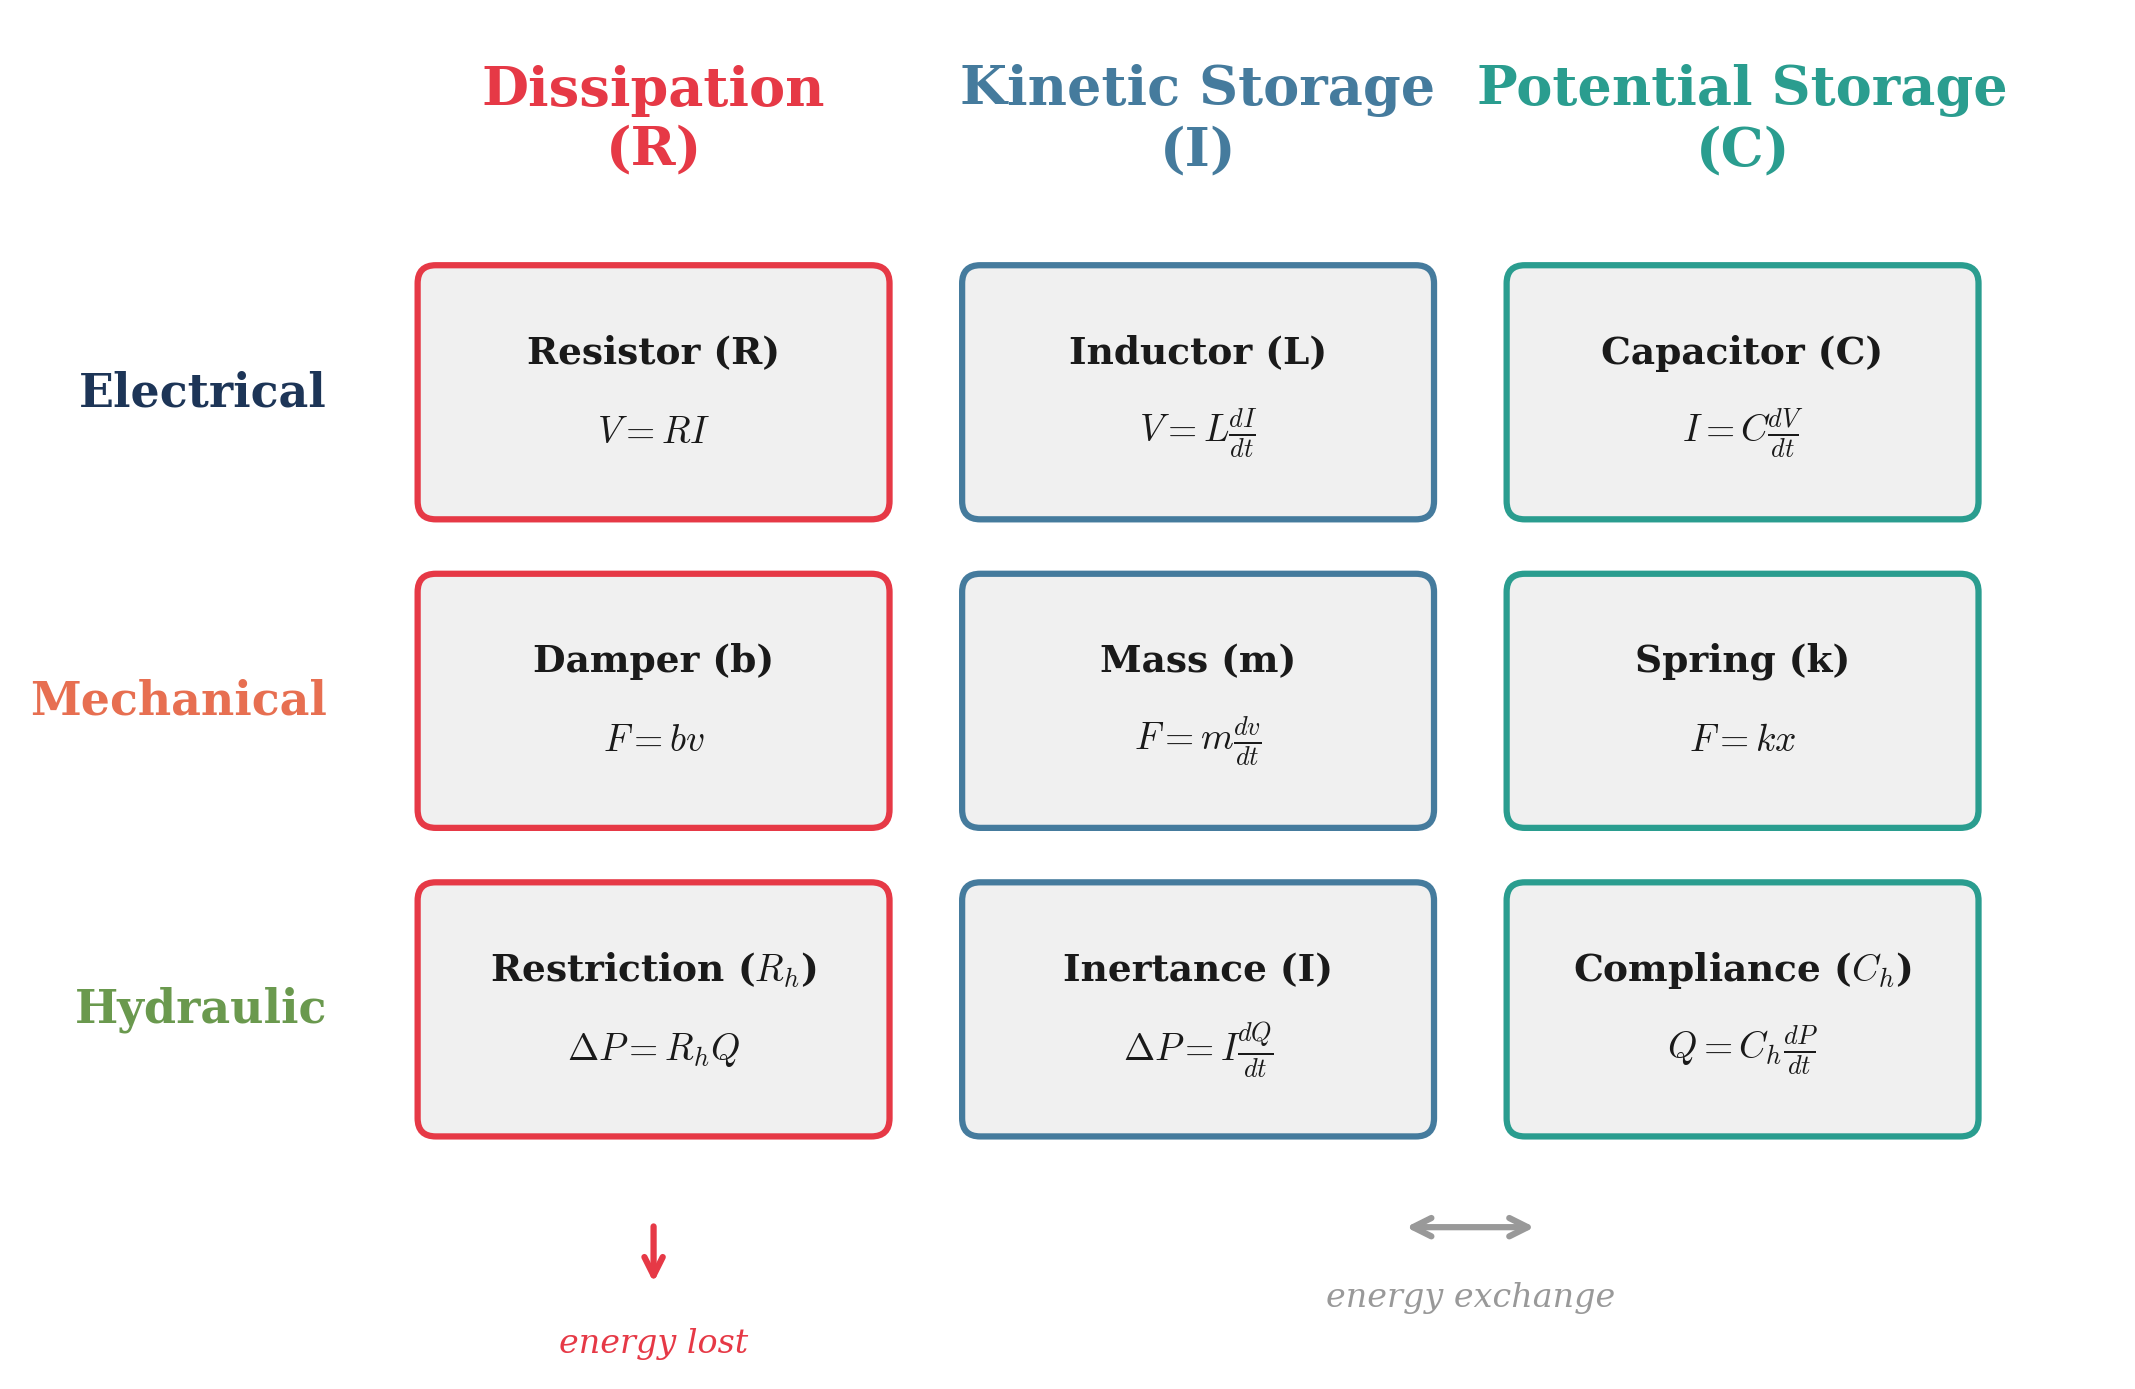
\includegraphics[width=0.9\linewidth,height=\textheight,keepaspectratio]{figures/fig_F1_cross_domain_RIC.png}

}

\caption{\label{fig-ric}The three energy roles --- dissipation (R),
kinetic storage (I), and potential storage (C) --- mapped across
electrical, mechanical, and hydraulic domains. Each column shares a
constitutive law structure; each row instantiates it with
domain-specific elements.}

\end{figure}%

\subsection{Effort, Flow, and the Constitutive
Laws}\label{effort-flow-and-the-constitutive-laws}

The mapping becomes concrete when writing the passive element laws in a
recognizable form. Each system has a paired set of terminal variables:
an \textbf{effort} variable (the driving difference) and a \textbf{flow}
variable (the through quantity). These terms --- and the classification
of passive elements into resistance, inertance, and compliance ---
originate from bond-graph theory, developed systematically by Paynter
(1961) and formalized as a modeling methodology by Karnopp, Margolis,
and Rosenberg (2012). The present treatment inherits their
classification and asks a different question: what does the universality
of this structure imply about the epistemology of dynamical modeling?

\textbf{Electrical:}

The electrical effort variable is voltage (\(V\)), and the flow variable
is current (\(I\)). The three passive circuit elements---resistor,
inductor, and capacitor---each relate these two variables through a
distinct constitutive law: proportionality, differentiation, or
integration.

\begin{itemize}
\item
  \textbf{Resistor:} \[V_R = RI\] where \(R\) is resistance, measured in
  Ohms (\(\Omega\)). Voltage drop is proportional to current. The faster
  charge flows, the more energy the resistor bleeds as heat.
\item
  \textbf{Inductor:} \[V_L = L\frac{dI}{dt}\] where \(L\) is inductance,
  measured in Henrys (H). Voltage is proportional to the \emph{rate of
  change} of current, not the quantity of current itself. The inductor
  stores energy in a magnetic field while current builds, then returns
  it as current collapses.
\item
  \textbf{Capacitor:} \[I_C = C\frac{dV}{dt}\] where \(C\) is
  capacitance, measured in Farads (F). Current flows into the capacitor
  only while its voltage is changing. Once fully charged, current stops.
  Energy is stored in the electric field between the plates, held in the
  separation of charge.
\end{itemize}

\textbf{Gravitational:}

The gravitational effort variable is potential (\(V_g\)), and the flow
variable is mass flow rate (\(\dot{m}\)). Gravitational potential is a
true potential --- energy per unit mass (J/kg) --- making it the closest
mechanical analog to voltage and pressure. The same three constitutive
forms apply:

\begin{itemize}
\item
  \textbf{Gravitational resistance} (drag / viscous friction on mass
  flow): \[V_g = R_g \dot{m}\] where \(R_g\) is gravitational
  resistance, measured in J·s/kg². Potential drop is proportional to
  mass flow rate. The faster mass flows through the resistive path, the
  more energy is lost.
\item
  \textbf{Gravitational inertance} (resistance to changes in mass flow):
  \[V_g = L_g \frac{d\dot{m}}{dt}\] where \(L_g\) is gravitational
  inertance, measured in J·s²/kg². Potential is proportional to the
  \emph{rate of change} of mass flow, not mass flow itself.
\item
  \textbf{Gravitational compliance} (mass storage under potential):
  \[\dot{m} = H \frac{dV_g}{dt}\] where \(H\) is gravitational
  compliance, measured in kg²/(J·s). Mass flow into storage is
  proportional to the rate of change of potential.
\end{itemize}

\textbf{Mechanical (translation):}

The mechanical effort variable is force (\(F\)), and the flow variable
is velocity (\(v = \dot{x}\)). The three passive mechanical
elements---damper, mass, and spring---each relate these two variables
through the same three constitutive forms: proportionality,
differentiation, or integration. Note that unlike voltage, pressure, and
gravitational potential, force is not a traditional potential --- it is
the gradient of potential energy with respect to displacement
(\(F = -dU/dx\)). Nevertheless, force carries units of energy per
displacement (J/m = N), and the effort-flow structure holds. The
familiar force laws (\(F = bv\), \(F = ma\), \(F = kx\)) can be
rewritten in effort-flow form: Newton's second law becomes
\(F = m\frac{dv}{dt}\) since \(a = \frac{dv}{dt}\), and Hooke's law
becomes \(v = \frac{1}{k}\frac{dF}{dt}\) after differentiating both
sides, where the compliance \(\frac{1}{k}\) plays the role of
capacitance.

\begin{itemize}
\item
  \textbf{Damper:} \[F_d = bv\] where \(b\) is the damping coefficient,
  measured in Newton-seconds per meter (N·s/m). Resistive force is
  proportional to velocity. The faster the mass moves, the harder the
  damper pushes back, converting kinetic energy to heat.
\item
  \textbf{Mass:} \[F_m = m\frac{dv}{dt}\] where \(m\) is mass, measured
  in kilograms (kg). Force is proportional to the \emph{rate of change}
  of velocity, not velocity itself. The mass does not resist motion---it
  resists \emph{changes} in motion (accelerations). A moving mass
  carries momentum past equilibrium, overshooting the spring's rest
  position and enabling oscillation.
\item
  \textbf{Spring:} \[v = \frac{1}{k}\frac{dF_s}{dt}\] where \(k\) is the
  spring stiffness, measured in Newtons per meter (N/m), and
  \(\frac{1}{k}\) is the mechanical compliance. Velocity is proportional
  to the rate of change of the restoring force. A softer spring (larger
  \(\frac{1}{k}\)) allows more velocity for the same rate of force
  change.
\end{itemize}

\begin{tcolorbox}[enhanced jigsaw, title=\textcolor{quarto-callout-note-color}{\faInfo}\hspace{0.5em}{Note}, breakable, left=2mm, opacitybacktitle=0.6, rightrule=.15mm, opacityback=0, toptitle=1mm, bottomrule=.15mm, arc=.35mm, leftrule=.75mm, colbacktitle=quarto-callout-note-color!10!white, toprule=.15mm, colframe=quarto-callout-note-color-frame, bottomtitle=1mm, titlerule=0mm, colback=white, coltitle=black]

The reader can verify that \textbf{mechanical rotation} follows the same
pattern with effort = torque \(\tau\) (J/rad) and flow = angular
velocity \(\omega\) (rad/s), yielding the constitutive laws
\(\tau = b_\theta \omega\), \(\tau = J\frac{d\omega}{dt}\), and
\(\omega = \frac{1}{k_\theta}\frac{d\tau}{dt}\).

\end{tcolorbox}

\textbf{Hydraulic:}

The hydraulic effort variable is pressure (\(p\)), and the flow variable
is volume flow rate (\(Q\)). The three passive hydraulic
elements---restriction, inertance, and compliance---each relate these
two variables through the same three constitutive forms:
proportionality, differentiation, or integration. The inertance of a
fluid column is \(I_h = \frac{\rho L}{A}\) (where \(\rho\) is density,
\(L\) is pipe length, and \(A\) is cross-sectional area), and the
compliance of an accumulator is \(C_h\), relating stored volume to
pressure via \(V_{\text{stored}} = C_h \, p\).

\begin{itemize}
\item
  \textbf{Restriction} (valve/orifice): \[p = R_h Q\] where \(R_h\) is
  hydraulic resistance, measured in Pascal-seconds per cubic meter
  (Pa·s/m³). Pressure drop is proportional to flow rate. The faster
  fluid moves through the restriction, the more energy is lost to
  viscous heating.
\item
  \textbf{Inertance} (long pipe / fluid slug): \[p = I_h \frac{dQ}{dt}\]
  where \(I_h\) is inertance, measured in Pascal-seconds-squared per
  cubic meter (Pa·s²/m³). Pressure is proportional to the \emph{rate of
  change} of flow, not flow itself. A long, narrow pipe resists rapid
  changes in flow rate---this is the mechanism behind water hammer.
\item
  \textbf{Compliance} (accumulator with flexible diaphragm):
  \[Q = C_h \frac{dp}{dt}\] where \(C_h\) is hydraulic compliance,
  measured in cubic meters per Pascal (m³/Pa). Flow into the accumulator
  is proportional to the rate of change of pressure. A more compliant
  accumulator accepts more flow for the same rate of pressure rise.
\end{itemize}

The structural correspondence across all domains is summarized below.

Role

Electrical

Gravitational

Mechanical

Hydraulic

Pattern

translation

rotation

Dissipation

\(V = RI\)

\(V_g = R_g \dot{m}\)

\(F = bv\)

\(\tau = b_\theta \omega\)

\(p = R_h Q\)

effort \(=\) resistance \(\times\) flow

Kinetic storage

\(V = L\frac{dI}{dt}\)

\(V_g = L_g \frac{d\dot{m}}{dt}\)

\(F = m\frac{dv}{dt}\)

\(\tau = J\frac{d\omega}{dt}\)

\(p = I_h \frac{dQ}{dt}\)

effort \(=\) inertance \(\times\) \(\frac{d}{dt}\)(flow)

Potential storage

\(I = C\frac{dV}{dt}\)

\(\dot{m} = H\frac{dV_g}{dt}\)

\(v = \frac{1}{k}\frac{dF}{dt}\)

\(\omega = \frac{1}{k_\theta}\frac{d\tau}{dt}\)

\(Q = C_h \frac{dp}{dt}\)

flow \(=\) compliance \(\times\) \(\frac{d}{dt}\)(effort)

Each row of the table compares a single shared statement:

\begin{itemize}
\tightlist
\item
  \textbf{Dissipation}: the dissipative element produces a response
  proportional to the flow variable --- an instantaneous, memoryless tax
  on any real process.
\item
  \textbf{Kinetic Storage}: the kinetic storage element resists changes
  in the flow variable --- energy carried in the momentum of the flow
  itself.
\item
  \textbf{Potential Storage}: the potential storage element resists
  further accumulation of the flow variable, producing a restoring
  effort that grows with the stored quantity --- energy held latent in
  configuration.
\end{itemize}

In every case, the same calculus applies --- proportionality,
differentiation, integration --- only the names and variables differ.

\begin{center}\rule{0.5\linewidth}{0.5pt}\end{center}

\section{Part IV: Impedance, Power, and Bond
Graphs}\label{part-iv-impedance-power-and-bond-graphs}

\subsection{Terminal Pairs}\label{terminal-pairs}

The constitutive laws were written in effort-flow form, but the effort
and flow variables were described by domain --- voltage and current,
force and velocity, etc. These variables have general dimensions. In
every domain, the effort variable carries units of energy per source,
and the flow variable carries units of source per time. Making this
explicit reveals why impedance and power take the same form everywhere.

The effort variable carries units of \textbf{energy per source}. In most
domains, this is a true potential:

\begin{itemize}
\tightlist
\item
  Electrical: voltage \(V\) --- energy per unit charge (J/C)
\item
  Gravitational: potential \(V_g\) --- energy per unit mass (J/kg)
\item
  Hydraulic: pressure \(p\) --- energy per unit volume (J/m³)
\end{itemize}

In mechanical systems, the effort variable has the same dimensional
structure but is not traditionally called a potential:

\begin{itemize}
\tightlist
\item
  Mechanical (translation): force \(F\) --- energy per unit displacement
  (J/m = N)
\item
  Mechanical (rotation): torque \(\tau\) --- energy per unit angle
  (J/rad)
\end{itemize}

Force and torque are gradients of potential energy with respect to their
source coordinates (\(F = -dU/dx\), \(\tau = -dU/d\theta\)), not
potentials themselves. The dimensional pattern --- energy per source ---
holds in every case, but the naming convention diverges for mechanical
systems.

The flow variable carries units of \textbf{source per time}:

\begin{itemize}
\tightlist
\item
  Electrical: current \(I\) --- charge per time (C/s = A)
\item
  Gravitational: mass flow rate \(\dot{m}\) --- mass per time (kg/s)
\item
  Hydraulic: volume flow rate \(Q\) --- volume per time (m³/s)
\item
  Mechanical (translation): velocity \(v\) --- displacement per time
  (m/s)
\item
  Mechanical (rotation): angular velocity \(\omega\) --- angle per time
  (rad/s)
\end{itemize}

The framework does not prescribe what the source must be; it requires
only that the effort-flow pairing be power-conjugate --- that their
product yield power. Different choices of ``source'' within the same
physical domain (e.g., displacement vs.~mass for mechanical systems)
yield different but equally valid descriptions.

These two generalized dimensions --- effort and flow --- combine to
produce two fundamental system quantities through division and
multiplication.

\textbf{Their ratio is impedance.} Dividing effort by flow:

\[Z = \frac{\text{effort}}{\text{flow}} = \frac{\text{energy}/\text{source}}{\text{source}/\text{time}} = \frac{\text{energy} \cdot \text{time}}{\text{source}^2}\]

Impedance encodes the dissipative and storage qualities of the system.
It controls how much driving difference is required per unit of through
quantity---how quickly energy is bled away relative to how much is
stored:

\begin{itemize}
\tightlist
\item
  Electrical:
  \(Z = \frac{V}{I} = \frac{\text{J/C}}{\text{C/s}} = \frac{\text{J} \cdot \text{s}}{\text{C}^2}\)
  (energy·time / charge²)
\item
  Gravitational:
  \(Z = \frac{V_g}{\dot{m}} = \frac{\text{J/kg}}{\text{kg/s}} = \frac{\text{J} \cdot \text{s}}{\text{kg}^2}\)
  (energy·time / mass²)
\item
  Mechanical (translation):
  \(Z = \frac{F}{v} = \frac{\text{J/m}}{\text{m/s}} = \frac{\text{J} \cdot \text{s}}{\text{m}^2}\)
  (energy·time / displacement²)
\item
  Mechanical (rotation):
  \(Z = \frac{\tau}{\omega} = \frac{\text{J/rad}}{\text{rad/s}} = \frac{\text{J} \cdot \text{s}}{\text{rad}^2}\)
  (energy·time / angle²)
\item
  Hydraulic:
  \(Z = \frac{p}{Q} = \frac{\text{J}/\text{m}^3}{\text{m}^3\text{/s}} = \frac{\text{J} \cdot \text{s}}{\text{m}^6}\)
  (energy·time / volume²)
\end{itemize}

Every domain reduces to the same generalized form --- the ``source''
differs (charge, displacement, angle, mass, volume), but the dimensional
structure is universal. Note that hydraulic pressure \(p\) denotes a
differential pressure --- the drop across the element measured with
respect to an absolute or gauge reference, analogous to voltage measured
with respect to ground.

\textbf{Their product is power.} Multiplying effort by flow:

\[P = \text{effort} \times \text{flow} = \frac{\text{energy}}{\text{source}} \times \frac{\text{source}}{\text{time}} = \frac{\text{energy}}{\text{time}}\]

The source units cancel, leaving power as the rate of energy
transfer---regardless of domain:

\begin{itemize}
\tightlist
\item
  Electrical: \(P = VI\) --- measured in Watts (W = J/s)
\item
  Gravitational: \(P = V_g \dot{m}\) --- measured in Watts
\item
  Mechanical (translation): \(P = Fv\) --- measured in Watts
\item
  Mechanical (rotation): \(P = \tau\omega\) --- measured in Watts
\item
  Hydraulic: \(P = p \cdot Q\) --- measured in Watts
\end{itemize}

Describing a system at its terminals using \((V, I)\) or \((F, v)\) or
\((V_g, \dot{m})\) or \((p, Q)\) makes it possible to directly track
\textbf{energy transfer}.

\begin{tcolorbox}[enhanced jigsaw, title=\textcolor{quarto-callout-tip-color}{\faLightbulb}\hspace{0.5em}{Tip}, breakable, left=2mm, opacitybacktitle=0.6, rightrule=.15mm, opacityback=0, toptitle=1mm, bottomrule=.15mm, arc=.35mm, leftrule=.75mm, colbacktitle=quarto-callout-tip-color!10!white, toprule=.15mm, colframe=quarto-callout-tip-color-frame, bottomtitle=1mm, titlerule=0mm, colback=white, coltitle=black]

\textbf{Why real sources ``sag under load.''} Real sources contain
internal dissipative effects, so part of the effort is spent internally
when the flow increases. A battery behaves like an EMF in series with
internal resistance: \(V_{\text{terminal}} = \mathcal{E} - rI\). A
pressurized canister behaves identically in hydraulics: reservoir
pressure is the available effort, but outlet pressure falls as flow
increases because pressure is lost across internal restrictions. Same
structure, different words and variables.

\end{tcolorbox}

\subsection{The Bridge to Dynamical
Systems}\label{the-bridge-to-dynamical-systems}

The moment a system includes storage --- something that accumulates over
time --- its behavior stops being a purely algebraic ratio at the
terminal and becomes an evolution law. Impedance is no longer a static
number; it becomes a dynamic, frequency-dependent quantity because part
of the effort is temporarily held in storage before being returned or
dissipated. That is where ordinary differential equations (and, when
storage is distributed in space, partial differential equations) enter
the conversation.

\begin{center}\rule{0.5\linewidth}{0.5pt}\end{center}

\section{Part V: The Complete Cross-Domain
Analogy}\label{part-v-the-complete-cross-domain-analogy}

Before developing the mathematical framework promised above, it is worth
consolidating everything established so far --- sources, displacements,
effort-flow pairs, power conjugacy, impedance, and storage elements ---
into a single reference. The following table organizes the cross-domain
analogies and will serve as the dictionary for the formal treatment that
follows in Part VI:

\begin{longtable}[]{@{}
  >{\raggedright\arraybackslash}p{(\linewidth - 10\tabcolsep) * \real{0.1667}}
  >{\raggedright\arraybackslash}p{(\linewidth - 10\tabcolsep) * \real{0.1667}}
  >{\raggedright\arraybackslash}p{(\linewidth - 10\tabcolsep) * \real{0.1667}}
  >{\raggedright\arraybackslash}p{(\linewidth - 10\tabcolsep) * \real{0.1667}}
  >{\raggedright\arraybackslash}p{(\linewidth - 10\tabcolsep) * \real{0.1667}}
  >{\raggedright\arraybackslash}p{(\linewidth - 10\tabcolsep) * \real{0.1667}}@{}}
\toprule\noalign{}
\begin{minipage}[b]{\linewidth}\raggedright
Component / Parameter
\end{minipage} & \begin{minipage}[b]{\linewidth}\raggedright
Gravitational
\end{minipage} & \begin{minipage}[b]{\linewidth}\raggedright
Electrical
\end{minipage} & \begin{minipage}[b]{\linewidth}\raggedright
Hydraulic
\end{minipage} & \begin{minipage}[b]{\linewidth}\raggedright
Mechanical (trans.)
\end{minipage} & \begin{minipage}[b]{\linewidth}\raggedright
Mechanical (rot.)
\end{minipage} \\
\midrule\noalign{}
\endhead
\bottomrule\noalign{}
\endlastfoot
\textbf{Source} & Mass \(m\) (kg) & Charge \(q\) (C) & Volume \(V\) (m³)
& Displacement \(x\) (m) & Angle \(\theta\) (rad) \\
\textbf{Displacement} & Height \(h\) & Path coordinate \(x\) & Volume
\(V\) & Position \(x\) & Angle \(\theta\) \\
\textbf{Motion} & Mass flow \(\dot{m}\) & Drift speed \(u_d\) & Volume
flow \(Q=\dot{V}\) & Velocity \(v=\dot{x}\) & Angular speed
\(\omega=\dot{\theta}\) \\
\textbf{Field} & Gravitic field \(g\) & Electric field \(E\) & Pressure
gradient \(-\nabla p\) & Acceleration \(a\) & Angular accel.
\(\alpha\) \\
\textbf{Force = Source·Field} & \(F=mg\) & \(F=qE\) & \(F=pA\) &
\(F=ma\)\textsuperscript{†} & \(\tau=J\alpha\)\textsuperscript{†} \\
\textbf{Work-Energy} & \(U=\int mg\,dh\) & \(U=\int V\,dq\) &
\(U=\int p\,dV\) & \(U=\int F\,dx\) & \(U=\int \tau\,d\theta\) \\
\textbf{Potential (energy/source)} & Grav. potential \(V_g=U/m=gh\)
(J/kg) & Voltage \(V=U/q\) (J/C) & Pressure \(p=U/V\) (J/m³) & Force
\(F\) (J/m) & Torque \(\tau\) (J/rad) \\
\textbf{Flux / Current (source/time)} & Mass flow \(\dot{m}\) (kg/s) &
\(I=\dot{q}\) (C/s) & \(Q=\dot{V}\) (m³/s) & \(v=\dot{x}\) (m/s) &
\(\omega=\dot{\theta}\) (rad/s) \\
\textbf{Power} & \(P=V_g \dot{m}\) & \(P=VI\) & \(P=p \cdot Q\) &
\(P=Fv\) & \(P=\tau\omega\) \\
\textbf{Impedance} & \(Z_g=V_g/\dot{m}\) & \(Z=V/I\) & \(Z=p/Q\) &
\(Z=F/v\) & \(Z=\tau/\omega\) \\
\textbf{Resistance (R-type)} & \(V_g=R_g \dot{m}\) Grav. resistance
\(R_g\) & \(V=RI\) Resistance \(R\) & \(p=R_h Q\) Hyd. resistance
\(R_h\) & \(F=bv\) Damping \(b\) & \(\tau=b_\theta\omega\) Rot. damping
\(b_\theta\) \\
\textbf{Conductance (G-type)} & \(G_g=1/R_g\) & \(G=1/R\) &
\(G_h=1/R_h\) & \(\mu=1/b\) & \(\mu_\theta=1/b_\theta\) \\
\textbf{Capacitance (C-type)} & \(m=HV_g\) Grav. capacitance \(H\) &
\(q=CV\) Capacitance \(C\) & \(V_{\text{stored}}=C_h p\) Hyd.
capacitance \(C_h\) & \(x=C_m F\) Compliance \(C_m=1/k\) &
\(\theta=C_\theta \tau\) Rot. compliance \(C_\theta=1/k_\theta\) \\
\textbf{Stiffness (inverse C)} & \(1/H\) & \(1/C\) & \(E_h=1/C_h\) &
\(k\) Spring constant & \(k_\theta\) \\
\textbf{Inductance (I-type)} & \(V_g=L_g\frac{d\dot{m}}{dt}\) Grav.
inductance \(L_g\) & \(V=L\dot{I}\) Inductance \(L\) & \(p=I_h\dot{Q}\)
Inertance \(I_h\) & \(F=m\dot{v}\) Mass \(m\) & \(\tau=J\dot{\omega}\)
Moment of inertia \(J\) \\
\textbf{C-state} (\(\int f\,dt\)) & Mass \(m\) & Charge \(q\) & Volume
\(V\) & Displacement \(x\) & Angle \(\theta\) \\
\textbf{I-state} (\(\int e\,dt\)) & Potential-impulse \(\pi_g\) & Flux
linkage \(\lambda\) & Pressure impulse \(\Pi\) & Momentum \(p\) &
Angular mom. \(L\) \\
\end{longtable}

\begin{tcolorbox}[enhanced jigsaw, title=\textcolor{quarto-callout-note-color}{\faInfo}\hspace{0.5em}{Note}, breakable, left=2mm, opacitybacktitle=0.6, rightrule=.15mm, opacityback=0, toptitle=1mm, bottomrule=.15mm, arc=.35mm, leftrule=.75mm, colbacktitle=quarto-callout-note-color!10!white, toprule=.15mm, colframe=quarto-callout-note-color-frame, bottomtitle=1mm, titlerule=0mm, colback=white, coltitle=black]

The \textbf{C-state} and \textbf{I-state} rows introduce the generalized
displacement and momentum variables used in bond-graph and Hamiltonian
formulations. These have not yet been discussed but are included here
for completeness; their meaning and significance will become clear in
the mathematical framework that follows.

\end{tcolorbox}

\textsuperscript{†} In the mechanical columns, acceleration \(a\) (and
angular acceleration \(\alpha\)) is not an independent environmental
field like \(g\) or \(E\); it is the kinematic result of the net force.
The Source · Field form is used here for structural consistency across
domains, but the causal arrow is reversed --- see the note in Part I.

The cross-domain analogies in this table are not merely pedagogical
heuristics; they are mathematical necessities --- consequences of power
conjugacy and conservation laws.

\begin{center}\rule{0.5\linewidth}{0.5pt}\end{center}

\section{Part VI: Mathematical
Framework}\label{part-vi-mathematical-framework}

\subsection{Finite-Dimensional Dynamical
Systems}\label{finite-dimensional-dynamical-systems}

Start with a forced mass-spring-damper system:

\[m\ddot{x} + b\dot{x} + kx = F(t)\]

where \(x(t)\) is position---an unknown function of time---\(m\), \(b\),
\(k\) are intrinsic parameters of the system (mass, damping, and
stiffness), and \(F(t)\) is an extrinsic time-dependent forcing
function.

\subsubsection{State-Space Formulation}\label{state-space-formulation}

To express this forced harmonic oscillator as a standard first-order
dynamical system, define the state vector:

\[z_1 = x, \qquad z_2 = \dot{x}, \qquad \mathbf{z} = \begin{pmatrix} z_1 \\ z_2 \end{pmatrix}\]

Taking derivatives:

\[\dot{z}_1 = \dot{x} = z_2, \qquad \dot{z}_2 = \ddot{x} = \frac{1}{m}\left(F(t) - bz_2 - kz_1\right)\]

As a system:

\[\dot{\mathbf{z}} = \begin{pmatrix} \dot{z}_1 \\ \dot{z}_2 \end{pmatrix} = \begin{pmatrix} z_2 \\ \frac{1}{m}F(t) - \frac{k}{m}z_1 - \frac{b}{m}z_2 \end{pmatrix}\]

Defining the intrinsic parameters as a vector \(\theta = (m, b, k)\),
the input driving force as \(u(t) = F(t)\), and the state vector as
\(\mathbf{z} = (z_1, z_2)\), and packing these all into one function:

\[\dot{\mathbf{z}} = f(\mathbf{z}, t; \theta, u(t)) = \begin{pmatrix} z_2 \\ -\frac{k}{m}z_1 - \frac{b}{m}z_2 + \frac{1}{m}u(t) \end{pmatrix}\]

Let the state be a point in the position-velocity plane,
\(\mathbf{z}(t) \in \mathbb{R}^2\). Separating the intrinsic linear
component from the extrinsic forcing component:

\[\dot{\mathbf{z}}(t) = \underbrace{\begin{pmatrix} 0 & 1 \\ -k/m & -b/m \end{pmatrix}}_{\mathbf{A}_\theta} \begin{pmatrix} z_1 \\ z_2 \end{pmatrix} + \underbrace{\begin{pmatrix} 0 \\ F(t)/m \end{pmatrix}}_{\mathbf{s}(t)}\]

The \textbf{intrinsic matrix} \(\mathbf{A}_\theta\) encodes the system's
own dynamics through its parameters, and \(\mathbf{s}(t)\) is the
\textbf{extrinsic forcing vector} (Figure~\ref{fig-state-space}). In
reduced form:

\[\dot{\mathbf{z}}(t) = \mathbf{A}_\theta \mathbf{z}(t) + \mathbf{s}(t)\]

\begin{figure}

\centering{

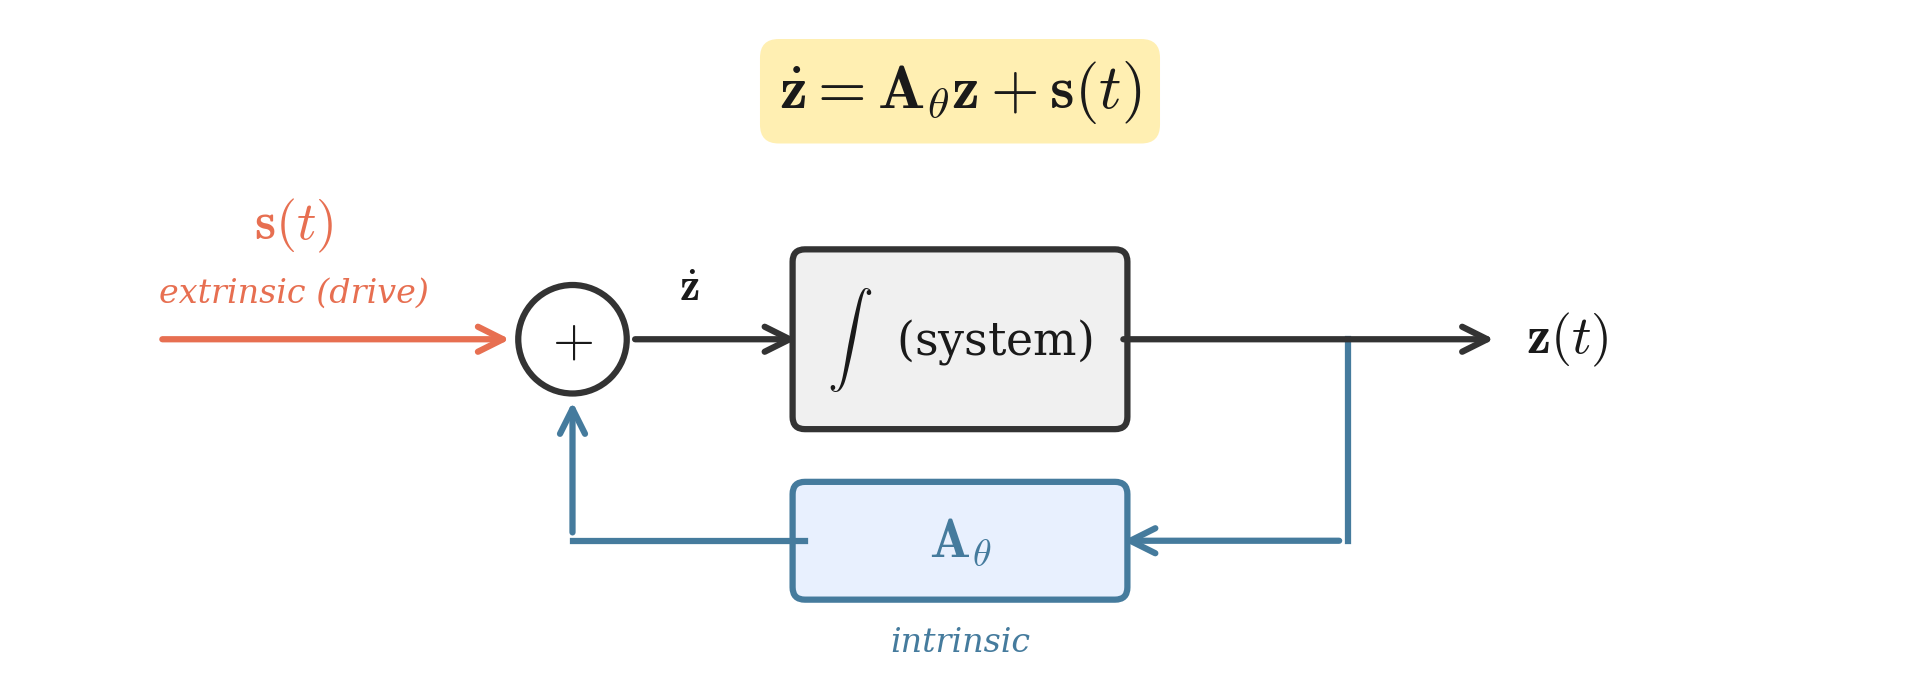
\includegraphics[width=0.85\linewidth,height=\textheight,keepaspectratio]{figures/fig_F3_state_space_block.png}

}

\caption{\label{fig-state-space}State-space block diagram. The intrinsic
matrix \(\mathbf{A}_\theta\) (blue, feedback) and the extrinsic forcing
\(\mathbf{s}(t)\) (orange, input) jointly determine the state trajectory
\(\mathbf{z}(t)\).}

\end{figure}%

\subsection{Chains of Coupled
Oscillators}\label{chains-of-coupled-oscillators}

To see how this structure scales beyond a single degree of freedom,
consider a chain of \(n\) masses connected by springs and dampers, with
positions \(x_i(t)\) and external forces \(F_i(t)\) for each mass \(i\).

\subsubsection{Matrix Formulation}\label{matrix-formulation}

Define the state vector by stacking all positions followed by all
velocities:

\[\mathbf{z} = \begin{pmatrix} \mathbf{x} \\ \dot{\mathbf{x}} \end{pmatrix} = [x_1, \ldots, x_n, \dot{x}_1, \ldots, \dot{x}_n]^T \in \mathbb{R}^{2n}\]

The intrinsic matrix takes the block form:

\[\mathbf{A}_\theta = \begin{pmatrix} \mathbf{0} & \mathbf{I} \\ -\mathbf{M}^{-1}\mathbf{K} & -\mathbf{M}^{-1}\mathbf{C} \end{pmatrix}\]

with \(\mathbf{0}\) and \(\mathbf{I}\) being \(n \times n\) zero and
identity matrices, \(\mathbf{M}\) a diagonal mass matrix, and
\(\mathbf{K}\) and \(\mathbf{C}\) the stiffness and damping matrices
respectively.

The \textbf{mass matrix} is diagonal:

\[\mathbf{M} = \begin{pmatrix} m_1 & 0 & \cdots & 0 \\ 0 & m_2 & \cdots & 0 \\ \vdots & \vdots & \ddots & \vdots \\ 0 & 0 & \cdots & m_n \end{pmatrix}\]

For identical masses, this reduces to \(\mathbf{M} = m\mathbf{I}\).

The \textbf{stiffness matrix}
\(\mathbf{K} \in \mathbb{R}^{n \times n}\), assuming each mass is
connected to its neighbors by springs of stiffness \(k_i\) and that the
first and last masses are connected to fixed walls (also by springs), is
tridiagonal:

\[\mathbf{K} = \begin{pmatrix} k_0 + k_1 & -k_1 & 0 & \cdots & 0 \\ -k_1 & k_1 + k_2 & -k_2 & \ddots & \vdots \\ 0 & -k_2 & k_2 + k_3 & \ddots & 0 \\ \vdots & \ddots & \ddots & \ddots & -k_{n-1} \\ 0 & \cdots & 0 & -k_{n-1} & k_{n-1} + k_n \end{pmatrix}\]

In index form:

\begin{itemize}
\tightlist
\item
  \(K_{ii} = k_{i-1} + k_i\), \(\;i = 1, \ldots, n\)
\item
  \(K_{i,i+1} = K_{i+1,i} = -k_i\), \(\;i = 1, \ldots, n-1\)
\item
  All other \(K_{ij} = 0\)
\end{itemize}

Were the masses influenced by the next-nearest neighbor, the matrix
would be pentadiagonal (springs between mass \(i\) and \(i+2\)). The
offset of a nonzero diagonal represents the proximity of physical
coupling between masses.

For identical springs \(k_i = k\), each diagonal entry becomes \(2k\)
and each off-diagonal becomes \(-k\).

The \textbf{damping matrix} \(\mathbf{C} \in \mathbb{R}^{n \times n}\)
has the same tridiagonal pattern with \(b\):

\[\mathbf{C} = \begin{pmatrix} b_0 + b_1 & -b_1 & 0 & \cdots & 0 \\ -b_1 & b_1 + b_2 & -b_2 & \ddots & \vdots \\ 0 & -b_2 & b_2 + b_3 & \ddots & 0 \\ \vdots & \ddots & \ddots & \ddots & -b_{n-1} \\ 0 & \cdots & 0 & -b_{n-1} & b_{n-1} + b_n \end{pmatrix}\]

In index form:

\begin{itemize}
\tightlist
\item
  \(C_{ii} = b_{i-1} + b_i\), \(\;i = 1, \ldots, n\)
\item
  \(C_{i,i+1} = C_{i+1,i} = -b_i\), \(\;i = 1, \ldots, n-1\)
\item
  All other \(C_{ij} = 0\)
\end{itemize}

For identical dampers \(b_i = b\), this simplifies analogously.

The extrinsic forcing vector collects all external driving forces:

\[\mathbf{s}(t) = \begin{pmatrix} \mathbf{0} \\ \mathbf{M}^{-1}\mathbf{F}(t) \end{pmatrix}, \qquad \mathbf{F}(t) = [F_1(t), \ldots, F_n(t)]^T\]

\subsubsection{Physical Interpretation}\label{physical-interpretation}

Now assume identical masses \(m\), identical springs of stiffness \(k\),
and identical dashpots of damping \(b\). For an interior mass \(i\), the
net spring force is \(k(x_{i-1} - 2x_i + x_{i+1})\) and the net damping
force is \(b(\dot{x}_{i-1} - 2\dot{x}_i + \dot{x}_{i+1})\). Newton's
second law gives:

\[m\ddot{x}_i = k(x_{i-1} - 2x_i + x_{i+1}) + b(\dot{x}_{i-1} - 2\dot{x}_i + \dot{x}_{i+1}) + F_i(t)\]

The coefficient pattern \((1, -2, 1)\) is the \textbf{discrete second
derivative stencil}---exactly the tridiagonal pattern encoded in
\(\mathbf{K}\) and \(\mathbf{C}\). The system again takes the form:

\[\dot{\mathbf{z}}(t) = \mathbf{A}_\theta \mathbf{z}(t) + \mathbf{s}(t)\]

\subsection{The Continuum Limit}\label{the-continuum-limit}

The nearest-neighbor chain already contains the spatial structure of a
one-dimensional elastic medium. The \((1, -2, 1)\) stencil in the
discrete equation is a finite-difference approximation to a second
spatial derivative---so as the number of masses grows and the spacing
shrinks, the chain should converge to a continuous wave equation.

To pass to a continuum, introduce a uniform spacing \(a\) between masses
and identify mass \(i\) with position \(x_i = i \cdot a\) along a
one-dimensional body. Approximate the discrete displacements by a smooth
field \(u(x,t)\) via \(x_i(t) \approx u(x_i, t)\), and relate the lumped
parameters to continuum quantities:

\begin{itemize}
\tightlist
\item
  Mass per unit length (\(\rho\) density, \(A\) cross-section):
  \(m = \rho A \, a\)
\item
  Axial stiffness (\(E\) Young's modulus): \(k = EA / a\)
\item
  Damping (\(\eta\) viscous coefficient): \(b = \eta A / a\)
\item
  Force per unit length: \(f(x_i, t) \approx F_i(t) / a\)
\end{itemize}

Substituting these into the discrete equation of motion and dividing by
\(a\):

\[\rho A \frac{\partial^2 u}{\partial t^2}\bigg|_{x_i} = EA \frac{u(x_{i+1}, t) - 2u(x_i, t) + u(x_{i-1}, t)}{a^2} + \eta A \frac{\dot{u}(x_{i+1}, t) - 2\dot{u}(x_i, t) + \dot{u}(x_{i-1}, t)}{a^2} + f(x_i, t)\]

The finite difference quotients

\[\frac{u(x_{i+1}, t) - 2u(x_i, t) + u(x_{i-1}, t)}{a^2} \;\longrightarrow\; \frac{\partial^2 u}{\partial x^2}\bigg|_{x_i}\]

(and the same for \(\dot{u}\)) are central second differences, which
converge to second spatial derivatives as \(a \to 0\). In the continuum
limit:

\[\rho A \frac{\partial^2 u}{\partial t^2} = EA \frac{\partial^2 u}{\partial x^2} + \eta A \frac{\partial^3 u}{\partial x^2 \partial t} + f(x,t)\]

Dividing by \(\rho A\) and defining:

\begin{itemize}
\tightlist
\item
  Wave speed: \(c^2 = E/\rho\)
\item
  Damping parameter: \(\gamma = \eta/\rho\)
\item
  Body-force term: \(g(x,t) = f(x,t)/(\rho A)\)
\end{itemize}

yields the \textbf{damped wave equation} of Kelvin-Voigt type (damping
proportional to strain rate \(\partial^2 u / \partial x \partial t\)):

\[\frac{\partial^2 u}{\partial t^2} = c^2 \frac{\partial^2 u}{\partial x^2} + \gamma \frac{\partial^3 u}{\partial x^2 \partial t} + g(x,t)\]

Setting \(\gamma = 0\) yields the \textbf{undamped wave equation}:

\[\frac{\partial^2 u}{\partial t^2} = c^2 \frac{\partial^2 u}{\partial x^2} + g(x,t)\]

with boundary conditions \(u(0,t) = u(L,t) = 0\) for a string of length
\(L = na\) with fixed ends.

The Kelvin-Voigt damping term
\(\gamma \, \partial^3 u / \partial x^2 \partial t\) arose because we
placed dashpots \emph{between} neighboring masses---dissipation through
spatial gradients in velocity. An alternative is \textbf{Rayleigh
damping}: if each mass instead has a dashpot to ground (force
\(-b\dot{x}_i\) rather than differences), the continuum damping term
becomes \(\gamma \, \partial u / \partial t\) rather than
\(\gamma \, \partial^3 u / \partial x^2 \partial t\), yielding:

\[\frac{\partial^2 u}{\partial t^2} + \gamma \frac{\partial u}{\partial t} = c^2 \frac{\partial^2 u}{\partial x^2} + g(x,t)\]

With free ends, the boundary conditions become
\(\partial u / \partial x |_{x=0} = \partial u / \partial x |_{x=L} = 0\).
The choice of damping model and boundary conditions reflects intrinsic
structural decisions about the physical system.

\subsection{Field Evolution as Operator
Equation}\label{field-evolution-as-operator-equation}

Introduce the first-order state field
\(\mathbf{w}(x,t) = (u(x,t),\; v(x,t))^T\) where
\(v(x,t) = \partial u / \partial t\). Then the wave equation becomes the
first-order system:

\[\frac{\partial u}{\partial t} = v, \qquad \frac{\partial v}{\partial t} = c^2 \frac{\partial^2 u}{\partial x^2} + \gamma \frac{\partial^3 u}{\partial x^2 \partial t} + g(x,t)\]

Setting \(\gamma = 0\) for a clean display, this can be written in
matrix form:

\[\frac{\partial}{\partial t} \begin{pmatrix} u \\ v \end{pmatrix} = \underbrace{\begin{pmatrix} 0 & 1 \\ c^2 \frac{\partial^2}{\partial x^2} & 0 \end{pmatrix}}_{\mathcal{L}_\theta} \begin{pmatrix} u \\ v \end{pmatrix} + \underbrace{\begin{pmatrix} 0 \\ g(x,t) \end{pmatrix}}_{\mathbf{S}(x,t)}\]

In reduced form:

\[\frac{\partial \mathbf{w}}{\partial t} = \mathcal{L}_\theta[\mathbf{w}] + \mathbf{S}(x,t)\]

The \textbf{intrinsic operator} \(\mathcal{L}_\theta\) is determined by:

\begin{itemize}
\tightlist
\item
  Material parameters \((E, \rho, \eta)\),
\item
  Geometry (string length, boundary conditions),
\item
  The choice of damping model (which would add terms to the lower-left
  and lower-right blocks).
\end{itemize}

The \textbf{extrinsic source} \(\mathbf{S}(x,t)\) encodes distributed
forcing along the string. This is exactly the field-level analogue of
the finite chain equation
\(\dot{\mathbf{z}} = \mathbf{A}_\theta \mathbf{z} + \mathbf{s}(t)\),
with \(\mathbf{A}_\theta\) replaced by \(\mathcal{L}_\theta\) and
\(\mathbf{s}(t)\) replaced by \(\mathbf{S}(x,t)\).

\begin{center}\rule{0.5\linewidth}{0.5pt}\end{center}

\section{Part VII: Conservation Laws and Constitutive
Relations}\label{part-vii-conservation-laws-and-constitutive-relations}

\subsection{The Two-Step Structure}\label{the-two-step-structure}

Part VI arrived at the general evolution equation
\(\frac{\partial \mathbf{w}}{\partial t} = \mathcal{L}_\theta[\mathbf{w}] + \mathbf{S}(x,t)\),
where the intrinsic operator \(\mathcal{L}_\theta\) and the extrinsic
source \(\mathbf{S}\) jointly determine the system's evolution. But
where does \(\mathcal{L}_\theta\) come from? How does one derive the
specific form of the operator for a given physical system?

Every evolution equation in the preceding table arises from a two-step
construction:

\begin{enumerate}
\def\labelenumi{\arabic{enumi}.}
\tightlist
\item
  \textbf{Write a conservation law} for the quantity of interest
  (energy, mass, charge, momentum).
\item
  \textbf{Insert a constitutive relation} that links the flux of that
  quantity to a driving gradient.
\end{enumerate}

Every conservation law takes the same form. If \(u\) is the density of
some conserved quantity and \(\mathbf{J}\) is the flux of that quantity
(flow per unit area), then:

\[\frac{\partial u}{\partial t} + \nabla \cdot \mathbf{J} = S\]

This says: the rate of change of \(u\) at a point equals the net flux
into that point, plus any local sources \(S\). The divergence operator
\(\nabla \cdot\) measures the net outflow of a vector field from a point
--- it is pure spatial bookkeeping, independent of any material. The
equation holds regardless of what \(u\) represents.

The constitutive relation closes the system by expressing the flux
\(\mathbf{J}\) in terms of the state:

\[\mathbf{J} = \underbrace{\text{Response}}_{\text{intrinsic}} \times \underbrace{\text{Drive}}_{\text{extrinsic}}\]

In the simplest (linear, isotropic) case, this is literal
multiplication: a material coefficient times a gradient. The gradient
operator \(\nabla\) measures the direction and rate of steepest increase
of the field variable --- again, purely geometric. What makes the
constitutive relation material-specific is the coefficient that
multiplies it. More generally, the ``Response'' may be a tensor, a
nonlinear function, or an operator with memory --- but the structural
pattern remains.

Substituting the constitutive relation into the conservation law closes
the system. In the simplest case --- a linear, isotropic constitutive
law \(\mathbf{J} = -\alpha \nabla u\) --- the substitution yields:

\[\frac{\partial u}{\partial t} = \alpha \nabla^2 u + S\]

where \(\nabla^2 = \nabla \cdot \nabla\) is the \textbf{Laplacian} ---
the divergence of the gradient. The Laplacian at a point measures how
much \(u\) there deviates from the average of its immediate
surroundings: it is positive where \(u\) sits in a local valley (lower
than its neighbors) and negative where \(u\) sits on a local peak.
Multiplied by the material coefficient \(\alpha\), it tells the system
how fast to equalize these spatial imbalances. The combined operator
\(\alpha \nabla^2\) \emph{is} the intrinsic operator
\(\mathcal{L}_\theta\) of Part VI.

This two-step procedure --- conservation law plus constitutive closure
--- is the standard derivation strategy across continuum mechanics and
transport theory (Bird, Stewart, and Lightfoot 2002). What is less
commonly emphasized is that the procedure is identical in every domain:
the same structural steps, applied to different conserved quantities and
material coefficients, produce every evolution equation in the table
below (Figure~\ref{fig-two-step}).

\begin{figure}

\centering{

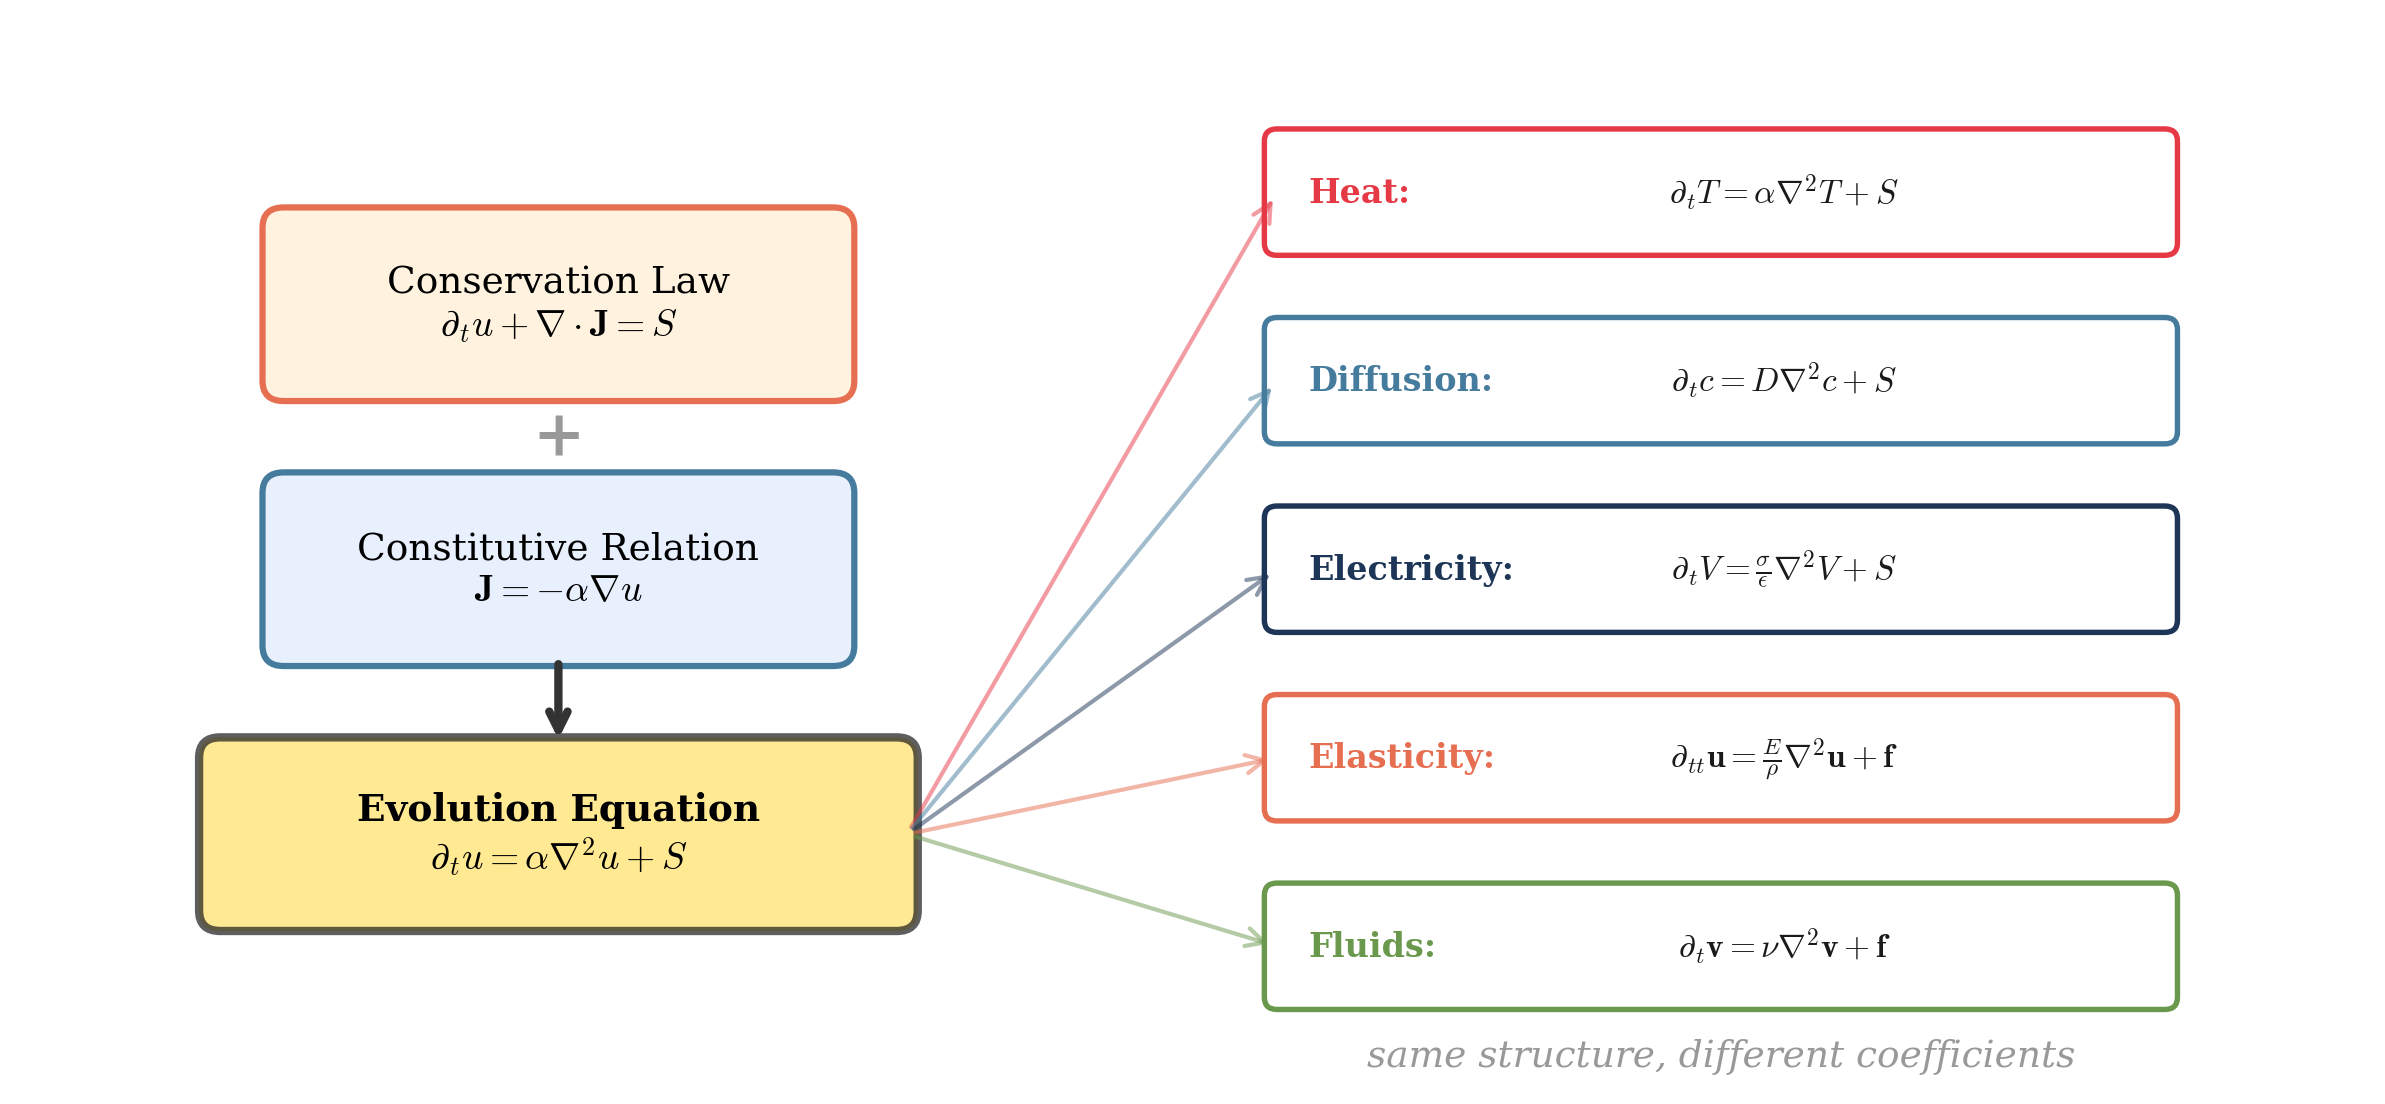
\includegraphics[width=0.9\linewidth,height=\textheight,keepaspectratio]{figures/fig_F5_two_step_construction.png}

}

\caption{\label{fig-two-step}The two-step construction: a conservation
law combined with a constitutive relation produces an evolution
equation. The same structure, with different material coefficients,
generates the governing PDE for each physical domain.}

\end{figure}%

The sections below demonstrate how this two-step procedure produces the
specific evolution equation for each physical domain.

\subsection{Heat Conduction}\label{heat-conduction}

A hot iron bar left in a cool room gradually equilibrates. Heat flows
from regions of high temperature to regions of low --- but \emph{how
fast} depends on the material. Copper equilibrates in seconds; ceramic
takes minutes. The two-step construction produces the evolution equation
governing this process.

\textbf{Conservation of energy.} In its most fundamental form, thermal
energy conservation states that the rate of change of energy density
\(e\) at a point equals the net heat flux into that point, plus any
local sources:

\[\frac{\partial e}{\partial t} + \nabla \cdot \mathbf{q} = Q\]

This equation is pure bookkeeping --- no material properties appear. It
holds for copper, water, air, or anything else. To rewrite it in terms
of the measurable quantity \emph{temperature}, one needs
\(de = \rho c_p \, dT\), where \(\rho\) is mass density and \(c_p\) is
specific heat capacity --- both material-dependent. This yields:

\[\rho c_p \frac{\partial T}{\partial t} + \nabla \cdot \mathbf{q} = Q\]

which has already absorbed one piece of material identity --- how
efficiently a substance stores thermal energy --- into the conservation
side. What the equation still does not specify is \emph{how} heat flows.
That is the job of the constitutive relation.

\textbf{Constitutive relation (Fourier's Law):}
\[\mathbf{q} = -k\nabla T\]

Heat flux flows down the temperature gradient. The thermal conductivity
\(k\) is the \emph{response}; the temperature gradient \(\nabla T\) is
the \emph{drive}. The negative sign ensures flux flows from hot to cold.

Substituting Fourier's Law into the conservation equation replaces
\(\mathbf{q}\) with \(-k\nabla T\), yielding
\(\nabla \cdot (k \nabla T)\). For a homogeneous material (\(k\)
constant), this simplifies to \(k \nabla^2 T\) --- the intrinsic
operator \(\mathcal{L}_\theta\) for heat conduction.

\textbf{Evolution equation (Heat equation):}
\[\frac{\partial T}{\partial t} = \alpha \nabla^2 T + \frac{Q}{\rho c_p}\]

where \(\alpha = k/(\rho c_p)\) is \textbf{thermal diffusivity}
{[}m²/s{]} --- a single number that absorbs all of the material's
intrinsic thermal properties.

\textbf{Conserved quantity:} thermal energy

\textbf{Intrinsic:} \(\alpha\) (thermal diffusivity --- how readily the
material conducts heat)

\textbf{Extrinsic:} \(Q\) (heat sources), boundary temperatures

\subsection{Mass Diffusion}\label{mass-diffusion}

A drop of ink in still water spreads over time. The ink molecules are
not pushed by any external force --- they wander randomly, colliding
with water molecules, and the statistical effect of these collisions is
a net flow from regions of high concentration to regions of low
concentration.

\textbf{Conservation of mass:}
\[\frac{\partial c}{\partial t} + \nabla \cdot \mathbf{J} = S\]

Unlike the heat case, no material conversion is needed --- concentration
\(c\) is already the natural field variable, and this conservation law
is material-independent.

\textbf{Constitutive relation (Fick's Law):} \[\mathbf{J} = -D\nabla c\]

Mass flux flows down the concentration gradient. The diffusivity \(D\)
{[}m²/s{]} is the \emph{response} --- it measures how easily molecules
move through the medium. The concentration gradient \(\nabla c\) is the
\emph{drive}. The structure is identical to Fourier's Law with \(D\)
playing the role of \(k\) and \(c\) playing the role of \(T\).

Substituting into the conservation law yields the same Laplacian
structure:

\textbf{Evolution equation (Diffusion equation):}
\[\frac{\partial c}{\partial t} = D\nabla^2 c + S\]

The heat equation and the diffusion equation share the same mathematical
form --- a shared structure that the two-step procedure, applied to
different conserved quantities, makes explicit.

\textbf{Conserved quantity:} mass (concentration \(c\))

\textbf{Intrinsic:} \(D\) (mass diffusivity --- how easily molecules
move through the medium)

\textbf{Extrinsic:} \(S\) (mass sources), boundary concentrations

\subsection{Charge Transport}\label{charge-transport}

Apply a voltage across a wire, and current flows. How much current
depends on the material: copper carries it freely; glass blocks it
almost entirely. The two-step construction applied to charge produces a
surprising result --- not diffusion, but exponential relaxation.

\textbf{Conservation of charge:}
\[\frac{\partial \rho_e}{\partial t} + \nabla \cdot \mathbf{J} = 0\]

Charge is strictly conserved --- there are no sources or sinks (unlike
heat, which can be generated internally). The right-hand side is zero.

\textbf{Constitutive relation (Ohm's Law):}
\[\mathbf{J} = \sigma \mathbf{E} = -\sigma \nabla V\]

Current density flows down the electric potential gradient. The
conductivity \(\sigma\) {[}S/m{]} is the \emph{response}; the electric
field \(\mathbf{E} = -\nabla V\) is the \emph{drive}. Once more, the
same structure: a material coefficient times a gradient.

Substituting Ohm's Law into the conservation equation replaces
\(\mathbf{J}\) with \(-\sigma \nabla V\):

\[\frac{\partial \rho_e}{\partial t} = \nabla \cdot (\sigma \nabla V)\]

For a homogeneous conductor (\(\sigma\) constant), this yields the
Laplacian \(\sigma \nabla^2 V\) --- the same spatial operator as in the
heat and diffusion equations. But closing the equation --- expressing
everything in terms of a single field variable --- requires a step with
no analog in the previous domains. The conserved quantity \(\rho_e\) and
the potential \(V\) are not related by a simple material conversion (as
\(e = \rho c_p T\) relates energy density to temperature); instead, they
are linked by a second physical law: Gauss's law,
\(\nabla^2 V = -\rho_e/\epsilon\), where \(\epsilon\) is the material
permittivity. Substituting eliminates \(V\):

\textbf{Evolution equation (Charge relaxation):}
\[\frac{\partial \rho_e}{\partial t} = -\frac{\sigma}{\epsilon}\,\rho_e\]

This is \emph{not} a diffusion equation. Free charge in a conductor
decays locally and exponentially, with time constant
\(\tau = \epsilon/\sigma\). For copper, \(\tau \approx 10^{-19}\) s ---
charge redistribution is effectively instantaneous. The intrinsic
operator is multiplication by \(-\sigma/\epsilon\): the two-step
procedure, applied to charge in a conductor, produces exponential
relaxation rather than spatial spreading. In the steady-state limit, the
conductor interior is charge-free and the potential satisfies Laplace's
equation \(\nabla^2 V = 0\) --- the same equation governing steady-state
temperature.

\textbf{Conserved quantity:} electric charge

\textbf{Intrinsic:} \(\sigma\) (conductivity), \(\epsilon\)
(permittivity) --- together determining the relaxation rate
\(\sigma/\epsilon\)

\textbf{Extrinsic:} applied voltages, boundary conditions

\subsection{Linear Elasticity}\label{linear-elasticity}

Strike a bell, and it rings. Pluck a guitar string, and it vibrates.
Deform any elastic solid, and internal stresses develop that resist the
deformation and, if released, drive the material back toward its rest
configuration. Unlike the previous three scalar-field examples,
elasticity involves a \emph{vector} field (displacement \(\mathbf{u}\))
and a constitutive relation linking a \emph{tensor} (stress) to a
\emph{tensor} (strain). The two-step pattern is the same, but the
algebra is richer.

\textbf{Conservation of momentum:}
\[\rho \frac{\partial^2 \mathbf{u}}{\partial t^2} = \nabla \cdot \boldsymbol{\sigma} + \mathbf{f}\]

This is Newton's Second Law applied to a continuous medium: mass density
times acceleration equals the divergence of the internal stress tensor
plus external body forces.

\textbf{Constitutive relation (Hooke's Law):}
\[\boldsymbol{\sigma} = \mathbf{C} : \boldsymbol{\varepsilon}\]

where \(\mathbf{C}\) is the fourth-order stiffness tensor and
\(\boldsymbol{\varepsilon} = \frac{1}{2}(\nabla\mathbf{u} + (\nabla\mathbf{u})^T)\)
is the strain tensor. Stress is proportional to strain --- the stiffness
tensor \(\mathbf{C}\) is the \emph{response}; the strain field
\(\boldsymbol{\varepsilon}\) is the \emph{drive}. For an isotropic
material, the 81 components of \(\mathbf{C}\) reduce to just two
independent constants (the Lamé parameters \(\lambda\) and \(\mu\)), but
the structural pattern is unchanged.

Substituting Hooke's Law into the momentum equation replaces
\(\boldsymbol{\sigma}\) with \(\mathbf{C} : \boldsymbol{\varepsilon}\).
For an isotropic material, the stress-strain relation simplifies to
\(\boldsymbol{\sigma} = \lambda(\nabla \cdot \mathbf{u})\mathbf{I} + 2\mu\boldsymbol{\varepsilon}\),
and taking the divergence yields
\((\lambda + \mu)\nabla(\nabla \cdot \mathbf{u}) + \mu\nabla^2\mathbf{u}\):

\textbf{Evolution equation (Navier equation):}
\[\rho \frac{\partial^2 \mathbf{u}}{\partial t^2} = (\lambda + \mu)\nabla(\nabla \cdot \mathbf{u}) + \mu\nabla^2\mathbf{u} + \mathbf{f}\]

The Laplacian reappears --- now acting on a vector field. The additional
term \((\lambda + \mu)\nabla(\nabla \cdot \mathbf{u})\) couples
compressional and shear deformations; it vanishes for incompressible
materials (\(\nabla \cdot \mathbf{u} = 0\)), reducing the equation to a
vector wave equation with shear wave speed \(c_s = \sqrt{\mu/\rho}\),
structurally identical to the scalar wave equation derived in Part VI.

\textbf{Conserved quantity:} momentum

\textbf{Intrinsic:} \(\mathbf{C}\) (material stiffness --- how strongly
the material resists deformation)

\textbf{Extrinsic:} \(\mathbf{f}\) (body forces), boundary loads and
displacements

\subsection{Fluid Mechanics}\label{fluid-mechanics}

Stir honey in a jar, then stop. The motion slows and eventually ceases
--- the honey's viscosity bleeds away kinetic energy as heat. Like
elasticity, fluid mechanics conserves momentum and involves tensor
stress. But fluids resist the \emph{rate} of deformation, not
deformation itself. A solid spring pushes back when stretched; a fluid
resists only while it is \emph{being} deformed.

\textbf{Conservation of momentum:}
\[\rho \frac{\partial \mathbf{v}}{\partial t} + \rho(\mathbf{v} \cdot \nabla)\mathbf{v} = \nabla \cdot \boldsymbol{\sigma} + \mathbf{f}\]

\textbf{Constitutive relation (Newton's Law of Viscosity):}
\[\boldsymbol{\sigma} = -p\mathbf{I} + \mu\left(\nabla \mathbf{v} + (\nabla \mathbf{v})^T\right)\]

For a Newtonian fluid, viscous stress is proportional to the rate of
strain. The dynamic viscosity \(\mu\) {[}Pa·s{]} is the \emph{response};
the velocity gradient \(\nabla \mathbf{v}\) is the \emph{drive}.

Substituting the constitutive relation into the momentum equation and
imposing the incompressibility constraint
(\(\nabla \cdot \mathbf{v} = 0\)) yields:

\textbf{Evolution equation (Navier--Stokes, incompressible):}
\[\rho \frac{\partial \mathbf{v}}{\partial t} + \rho(\mathbf{v} \cdot \nabla)\mathbf{v} = -\nabla p + \mu \nabla^2 \mathbf{v} + \mathbf{f}\]

The viscous term \(\mu\nabla^2\mathbf{v}\) has the same Laplacian
structure found in every preceding domain. Dividing through by \(\rho\)
isolates the kinematic viscosity \(\nu = \mu/\rho\) {[}m²/s{]} --- the
direct fluid analog of thermal diffusivity \(\alpha\) and mass
diffusivity \(D\). All three carry units of m²/s and play the same
mathematical role: they set the rate at which spatial gradients smooth
out.

\textbf{Conserved quantity:} momentum

\textbf{Intrinsic:} \(\mu\) (dynamic viscosity --- how strongly the
fluid resists shearing), \(\rho\) (density)

\textbf{Extrinsic:} \(\mathbf{f}\) (body forces), pressure gradients,
boundary velocities

\begin{tcolorbox}[enhanced jigsaw, title=\textcolor{quarto-callout-important-color}{\faExclamation}\hspace{0.5em}{Important}, breakable, left=2mm, opacitybacktitle=0.6, rightrule=.15mm, opacityback=0, toptitle=1mm, bottomrule=.15mm, arc=.35mm, leftrule=.75mm, colbacktitle=quarto-callout-important-color!10!white, toprule=.15mm, colframe=quarto-callout-important-color-frame, bottomtitle=1mm, titlerule=0mm, colback=white, coltitle=black]

\textbf{A critical distinction.} The Navier--Stokes equation contains
the nonlinear advection term
\(\rho(\mathbf{v} \cdot \nabla)\mathbf{v}\), which has no analog in the
previous examples. This term means the velocity field advects
\emph{itself} --- the fluid's own motion alters the forces it
experiences. The constitutive relation (Newton's law of viscosity) is
still linear, but the overall evolution equation is not. This is where
the linear ``Response × Drive'' framework meets its limits --- a theme
beyond the scope of the present treatment.

\end{tcolorbox}

\subsection{The Pattern Summarized}\label{the-pattern-summarized}

\begin{longtable}[]{@{}
  >{\raggedright\arraybackslash}p{(\linewidth - 10\tabcolsep) * \real{0.1667}}
  >{\raggedright\arraybackslash}p{(\linewidth - 10\tabcolsep) * \real{0.1667}}
  >{\raggedright\arraybackslash}p{(\linewidth - 10\tabcolsep) * \real{0.1667}}
  >{\raggedright\arraybackslash}p{(\linewidth - 10\tabcolsep) * \real{0.1667}}
  >{\raggedright\arraybackslash}p{(\linewidth - 10\tabcolsep) * \real{0.1667}}
  >{\raggedright\arraybackslash}p{(\linewidth - 10\tabcolsep) * \real{0.1667}}@{}}
\toprule\noalign{}
\begin{minipage}[b]{\linewidth}\raggedright
Domain
\end{minipage} & \begin{minipage}[b]{\linewidth}\raggedright
Conserved Quantity
\end{minipage} & \begin{minipage}[b]{\linewidth}\raggedright
Constitutive Law
\end{minipage} & \begin{minipage}[b]{\linewidth}\raggedright
Response (Intrinsic)
\end{minipage} & \begin{minipage}[b]{\linewidth}\raggedright
Evolution Coefficient
\end{minipage} & \begin{minipage}[b]{\linewidth}\raggedright
Drive (Extrinsic)
\end{minipage} \\
\midrule\noalign{}
\endhead
\bottomrule\noalign{}
\endlastfoot
Heat & Energy & Fourier & \(k\) (conductivity) & \(\alpha = k/\rho c_p\)
(thermal diffusivity) {[}m²/s{]} & \(\nabla T\) (temperature
gradient) \\
Diffusion & Mass & Fick & \(D\) (diffusivity) & \(D\) (mass diffusivity)
{[}m²/s{]} & \(\nabla c\) (concentration gradient) \\
Electricity & Charge & Ohm & \(\sigma\) (conductivity) &
\(\sigma/\epsilon\) (charge relaxation rate) {[}1/s{]} & \(\mathbf{E}\)
(electric field) \\
Elasticity & Momentum & Hooke & \(\mathbf{C}\) (stiffness) &
\(c_s^2 = \mu/\rho\) (shear wave speed²) {[}m²/s²{]} &
\(\boldsymbol{\varepsilon}\) (strain tensor) \\
Fluids & Momentum & Newton & \(\mu\) (viscosity) & \(\nu = \mu/\rho\)
(kinematic viscosity) {[}m²/s{]} & \(\nabla \mathbf{v}\) (velocity
gradient) \\
\end{longtable}

The conservation law is always the same abstract statement: ``the rate
of change equals the net inflow plus sources.'' What distinguishes one
field from another is the constitutive relation --- the specific form of
the Response × Drive product. The material coefficient (conductivity,
diffusivity, stiffness, viscosity) encodes the system's intrinsic
character; the gradient or field encodes the extrinsic drive. The
evolution coefficient --- obtained by combining the constitutive
parameter with material density or capacity --- is the quantity that
actually governs the dynamics. For heat, diffusion, and fluids, this
coefficient carries units of m²/s and sets the rate at which spatial
gradients smooth out; for electricity it is a relaxation rate; for
elasticity it is a squared wave speed.

\begin{center}\rule{0.5\linewidth}{0.5pt}\end{center}

\section{Part VIII: Spectral Geometry and the State
Manifold}\label{part-viii-spectral-geometry-and-the-state-manifold}

\subsection{From Fields to Geometry}\label{from-fields-to-geometry}

Part VII showed that a two-step construction --- conservation law plus
constitutive relation --- produces evolution equations across every
physical domain. But what is the nature of the mathematical object that
evolves? In Part I, a mass or charge was a single object with a position
and velocity. In Part VI, we generalized to chains of \(n\) coupled
oscillators described by a state vector
\(\mathbf{z} \in \mathbb{R}^{2n}\), then passed to the continuum limit,
where the state became an entire field \(u(x,t)\) --- a function defined
over space. At each instant, the ``state'' of a heat-conducting rod is
not a number but a \emph{temperature profile}: a point in an
infinite-dimensional function space.

This section makes that picture rigorous and extracts its geometric
content. The key insight: every concept from finite-dimensional
dynamical systems --- state spaces, trajectories, stability, invariant
structures --- survives the passage to infinite dimensions. A PDE is an
ODE on a function space.

\subsection{The State Manifold}\label{the-state-manifold}

Part VI established that a PDE of the form
\(\frac{\partial u}{\partial t} = \mathcal{L}_\theta[u] + S(x,t)\) can
be written as an abstract evolution equation on a Hilbert space \(H\)
(Pazy 1983) (typically \(L^2(\Omega)\), the space of square-integrable
functions on the spatial domain \(\Omega\)):

\[\frac{d\mathbf{u}}{dt} = \mathbf{A}\mathbf{u} + \mathbf{S}(t), \quad \mathbf{u}(0) = \mathbf{u}_0\]

where \(\mathbf{u}(t) \in H\) is the field configuration,
\(\mathbf{A}: D(\mathbf{A}) \subset H \to H\) is the intrinsic operator,
and \(\mathbf{S}(t) \in H\) is the extrinsic source (the
functional-analytic foundations follow from standard semigroup theory;
see Pazy, 1983). The space \(H\) is the \textbf{state manifold} --- each
point represents one possible field configuration, and the operator
\(\mathbf{A}\) defines a vector field on this manifold, assigning to
each configuration a direction and rate of change. A trajectory
\(\mathbf{u}(t)\) is a curve through this space, traced out as the
system evolves. The spectral decomposition of such operators is also the
central object of the Koopman operator program (Mezić 2020; Brunton et
al. 2022), which pursues data-driven identification of these intrinsic
spectral structures; the present treatment derives the same
decomposition from first principles via the conservation-law
construction.

In finite dimensions, the state manifold is \(\mathbb{R}^{2n}\) --- the
phase space of positions and velocities. In the continuum limit, it
becomes infinite-dimensional, but its role is identical: it is the space
on which the operator acts, and its geometry is determined by the
intrinsic operator.

\subsection{The Spectral
Decomposition}\label{the-spectral-decomposition}

The intrinsic operator \(\mathbf{A}\) determines the \textbf{geometry}
of the state manifold --- the directions in which the system naturally
moves, how fast, and whether perturbations grow or decay.

\textbf{Eigenfunctions (Modes).} Solutions to
\(\mathbf{A}\phi_n = \lambda_n\phi_n\) represent the natural shapes the
system tends to assume. Under suitable conditions (compact,
self-adjoint, or sectorial operators), these eigenfunctions form an
orthonormal basis for \(H\), so that any state can be expanded as
\(\mathbf{u} = \sum_n c_n \phi_n\).

\textbf{Eigenvalues (Rates).} The spectrum
\(\sigma(\mathbf{A}) = \{\lambda_n\}\) determines the fate of each mode:

\begin{itemize}
\tightlist
\item
  \(\text{Re}(\lambda_n) < 0\): mode \(\phi_n\) \textbf{decays} at rate
  \(e^{\text{Re}(\lambda_n) t}\)
\item
  \(\text{Re}(\lambda_n) > 0\): mode \(\phi_n\) \textbf{grows} at rate
  \(e^{\text{Re}(\lambda_n) t}\)
\item
  \(\text{Im}(\lambda_n) \neq 0\): mode \(\phi_n\) \textbf{oscillates}
  at frequency \(|\text{Im}(\lambda_n)|\)
\end{itemize}

\textbf{Invariant subspaces.} The spectrum partitions the state manifold
into three invariant subspaces:

\begin{itemize}
\tightlist
\item
  The \textbf{stable subspace} \(E^s\): the span of all eigenfunctions
  with \(\text{Re}(\lambda_n) < 0\). Perturbations in these directions
  decay.
\item
  The \textbf{unstable subspace} \(E^u\): the span of all eigenfunctions
  with \(\text{Re}(\lambda_n) > 0\). Perturbations in these directions
  grow.
\item
  The \textbf{center subspace} \(E^c\): the span of all eigenfunctions
  with \(\text{Re}(\lambda_n) = 0\). Perturbations neither grow nor
  decay; their fate is governed by nonlinear effects beyond the linear
  framework.
\end{itemize}

The system is \textbf{globally stable} if and only if \(E^u\) is empty
--- every eigenvalue has negative real part, and every perturbation
eventually decays. This geometric structure is built entirely from
intrinsic properties (material parameters, domain shape, boundary
conditions) and exists independently of any particular trajectory.

\subsubsection{\texorpdfstring{Example: Heat Equation on
\([0,1]\)}{Example: Heat Equation on {[}0,1{]}}}\label{example-heat-equation-on-01}

The heat equation
\(\frac{\partial u}{\partial t} = \alpha \frac{\partial^2 u}{\partial x^2}\)
on \([0,1]\) with Dirichlet boundary conditions
(\(u(0,t) = u(1,t) = 0\)) makes the spectral picture concrete:

\begin{itemize}
\tightlist
\item
  \textbf{Eigenfunctions:} \(\phi_n(x) = \sin(n\pi x)\) for
  \(n = 1, 2, 3, \ldots\)
\item
  \textbf{Eigenvalues:} \(\lambda_n = -\alpha(n\pi)^2\)
\end{itemize}

Every eigenvalue is negative and real: the stable subspace is the entire
state space, the unstable and center subspaces are empty, and there are
no oscillations. High-frequency modes (large \(n\)) decay far faster
than low-frequency modes --- this is why heat diffusion smooths sharp
features: it rapidly kills high-\(n\) content while the fundamental mode
\(\sin(\pi x)\) persists longest.

Any initial temperature profile \(u_0(x)\) decomposes as
\(u_0 = \sum_n c_n \sin(n\pi x)\), and the solution is:

\[u(x,t) = \sum_n c_n \, e^{-\alpha n^2 \pi^2 t} \sin(n\pi x)\]

Consider two different initial profiles: a triangular peak centered at
\(x = 1/2\), and a step function on \([1/4, 3/4]\). Both decompose into
the same eigenfunctions, but with different coefficients \(c_n\). Their
transient evolutions are visibly different --- the step function
develops Gibbs-like oscillations before smoothing, while the triangular
peak decays more uniformly. Yet both converge to the \emph{same}
long-time behavior: exponential decay dominated by the slowest mode,
\(c_1 \, e^{-\alpha\pi^2 t}\sin(\pi x)\). The intrinsic operator
determines the landscape --- which modes exist, which decay fastest,
what the long-time limit looks like. The initial condition selects which
path through that landscape is actually traversed.

\subsection{Trajectories as Realized
Histories}\label{trajectories-as-realized-histories}

The spectral decomposition cleanly separates what is determined by
intrinsic structure from what requires extrinsic specification.

\textbf{The operator \(\mathbf{A}\) determines the landscape:}

\begin{itemize}
\tightlist
\item
  Which directions in state space are stable, unstable, or neutral
\item
  The decay and oscillation rates of each mode
\item
  The long-time attractors (steady states, limit cycles)
\item
  The qualitative character of all possible trajectories
\end{itemize}

\textbf{Initial conditions and forcing select the path:}

\begin{itemize}
\tightlist
\item
  \textbf{Initial conditions \(\mathbf{u}_0\)} determine the starting
  point on the manifold. The modal expansion
  \(\mathbf{u}_0 = \sum_n c_n \phi_n\) distributes the initial state's
  energy across the intrinsic directions --- and therefore determines
  which modes are excited and how strongly.
\item
  \textbf{Forcing \(\mathbf{S}(t)\)} injects energy into particular
  modes, pushing the system away from its natural relaxation. A
  spatially uniform heat source excites all symmetric modes; a
  sinusoidal source targets a specific one.
\item
  \textbf{Boundary conditions} constrain which eigenfunctions are
  admissible, restricting the accessible region of the manifold.
  Dirichlet conditions (\(u = 0\) at the boundary) and Neumann
  conditions (\(\partial u/\partial n = 0\)) yield different
  eigenfunction families and different spectral geometries.
\end{itemize}

The operator \(\mathbf{A}\) carves the landscape; initial data
\(\mathbf{u}_0\) and forcing \(\mathbf{S}(t)\) select which path through
that landscape is actually realized (Figure~\ref{fig-spectral}). This
separation --- geometry from history, intrinsic from extrinsic --- is
the central structural fact that Part IX now exploits.

\begin{figure}

\centering{

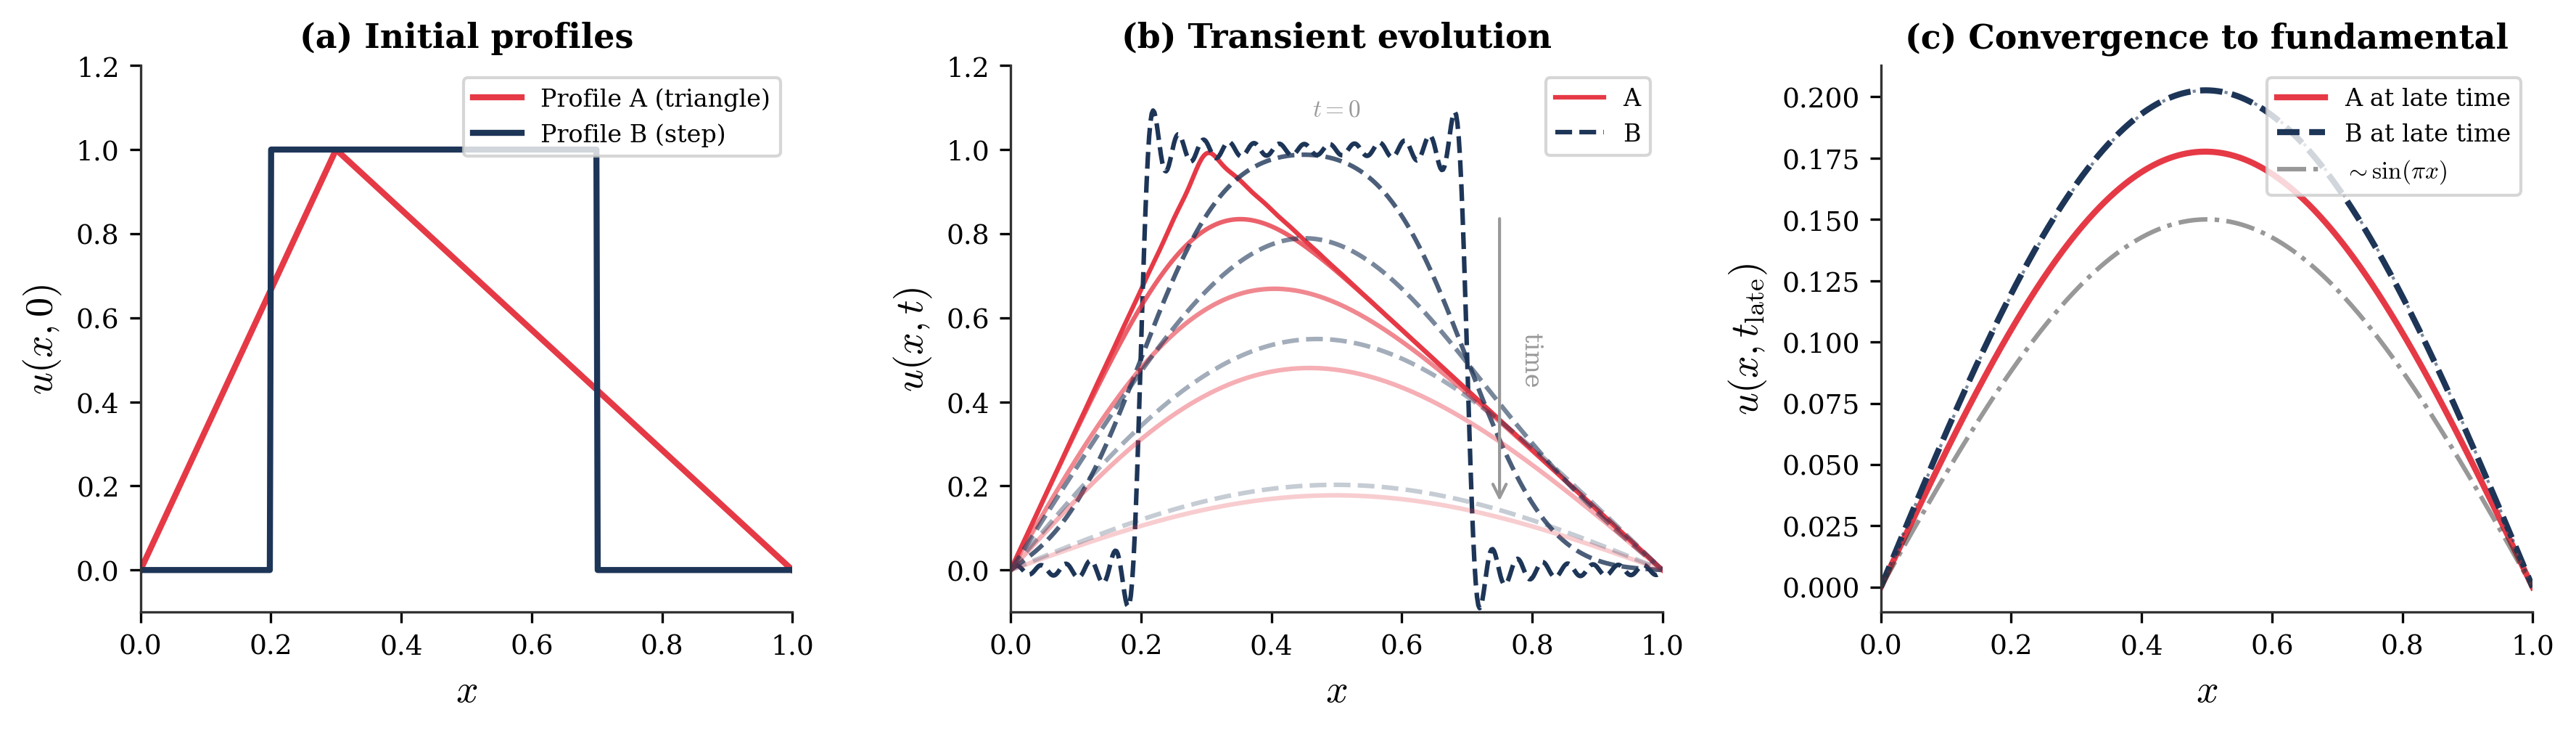
\includegraphics[width=1\linewidth,height=\textheight,keepaspectratio]{figures/fig_F2_heat_spectral.png}

}

\caption{\label{fig-spectral}Heat equation spectral example. (a) Two
different initial temperature profiles --- a triangular peak and a step
function. (b) Both profiles evolve under the same diffusion operator,
with higher modes decaying fastest. (c) At late times, both converge to
the fundamental mode \(\sin(\pi x)\), differing only in amplitude. The
intrinsic operator determines the landscape; initial conditions select
the path.}

\end{figure}%

\begin{center}\rule{0.5\linewidth}{0.5pt}\end{center}

\section{Part IX: Causal Attribution and the Underdetermination
Theorem}\label{part-ix-causal-attribution-and-the-underdetermination-theorem}

\subsection{The Product Structure at Every
Level}\label{the-product-structure-at-every-level}

The interaction between intrinsic and extrinsic factors --- the central
motif of this framework --- creates a fundamental epistemic barrier. At
every level of description developed so far, observable behavior is
generated by the joint action of response and drive:

\begin{itemize}
\tightlist
\item
  \textbf{Constitutive:} \(\mathbf{J} = \sigma \mathbf{E}\),
  \(\mathbf{q} = -k\nabla T\),
  \(\boldsymbol{\sigma} = \mathbf{C}:\boldsymbol{\varepsilon}\) (Part
  VII)
\item
  \textbf{Finite-dimensional:}
  \(\dot{\mathbf{z}} = \mathbf{A}_\theta \mathbf{z} + \mathbf{s}(t)\)
  (Part VI)
\item
  \textbf{Operator:}
  \(\frac{d\mathbf{u}}{dt} = \mathbf{A}\mathbf{u} + \mathbf{S}(t)\)
  (Part VIII)
\end{itemize}

At each level, observing the output alone cannot uniquely determine the
individual contributions of the intrinsic and extrinsic factors. This
section formalizes why.

\subsection{Scalar Underdetermination}\label{scalar-underdetermination}

The simplest case: given a scalar observation \(B = R \times D\), any
rescaling

\[B = (\alpha R) \times \left(\frac{D}{\alpha}\right), \quad \alpha \neq 0\]

produces the same \(B\). One equation, two unknowns --- the
factorization is structurally underdetermined. This is not a statement
about measurement noise or experimental difficulty. It is an algebraic
fact: the product carries less information than its factors.

\subsection{Operator-Level
Underdetermination}\label{operator-level-underdetermination}

The ambiguity persists --- and deepens --- at the level of field
evolution. Suppose we observe a complete trajectory \(\mathbf{u}(t)\)
satisfying

\[\frac{d\mathbf{u}}{dt} = \mathbf{A}\mathbf{u} + \mathbf{S}(t)\]

For \emph{any} alternative operator \(\mathbf{A}'\), the forcing

\[\mathbf{S}'(t) = \frac{d\mathbf{u}}{dt} - \mathbf{A}'\mathbf{u}(t)\]

produces the \emph{identical} trajectory. Different intrinsic structure
combined with different extrinsic drives yields the same observed
history. The trajectory constrains the \emph{sum}
\(\mathbf{A}\mathbf{u} + \mathbf{S}\), never the summands individually.

Concretely: a heat-conducting rod with high thermal diffusivity
\(\alpha\) and weak internal heating can produce the same temperature
record \(T(x,t)\) as a rod with low diffusivity and strong heating. From
the temperature history alone --- even a perfect, noiseless record ---
one cannot determine which scenario obtained. The spectral geometry of
Part VIII (eigenfunctions, decay rates, invariant subspaces) is entirely
invisible to an observer who does not independently know the intrinsic
operator.

In matrix notation (Part VI), the same argument takes a multiplicative
form:
\(\mathbf{J} = \mathbf{L} \cdot \mathbf{X} = (\mathbf{L}\mathbf{M}) \cdot (\mathbf{M}^{-1}\mathbf{X})\)
for any invertible \(\mathbf{M}\). The group of invertible
transformations acts on the (response, drive) pair while leaving the
observable invariant --- a symmetry that no amount of output data can
break (Figure~\ref{fig-underdetermination}).

\begin{figure}

\centering{

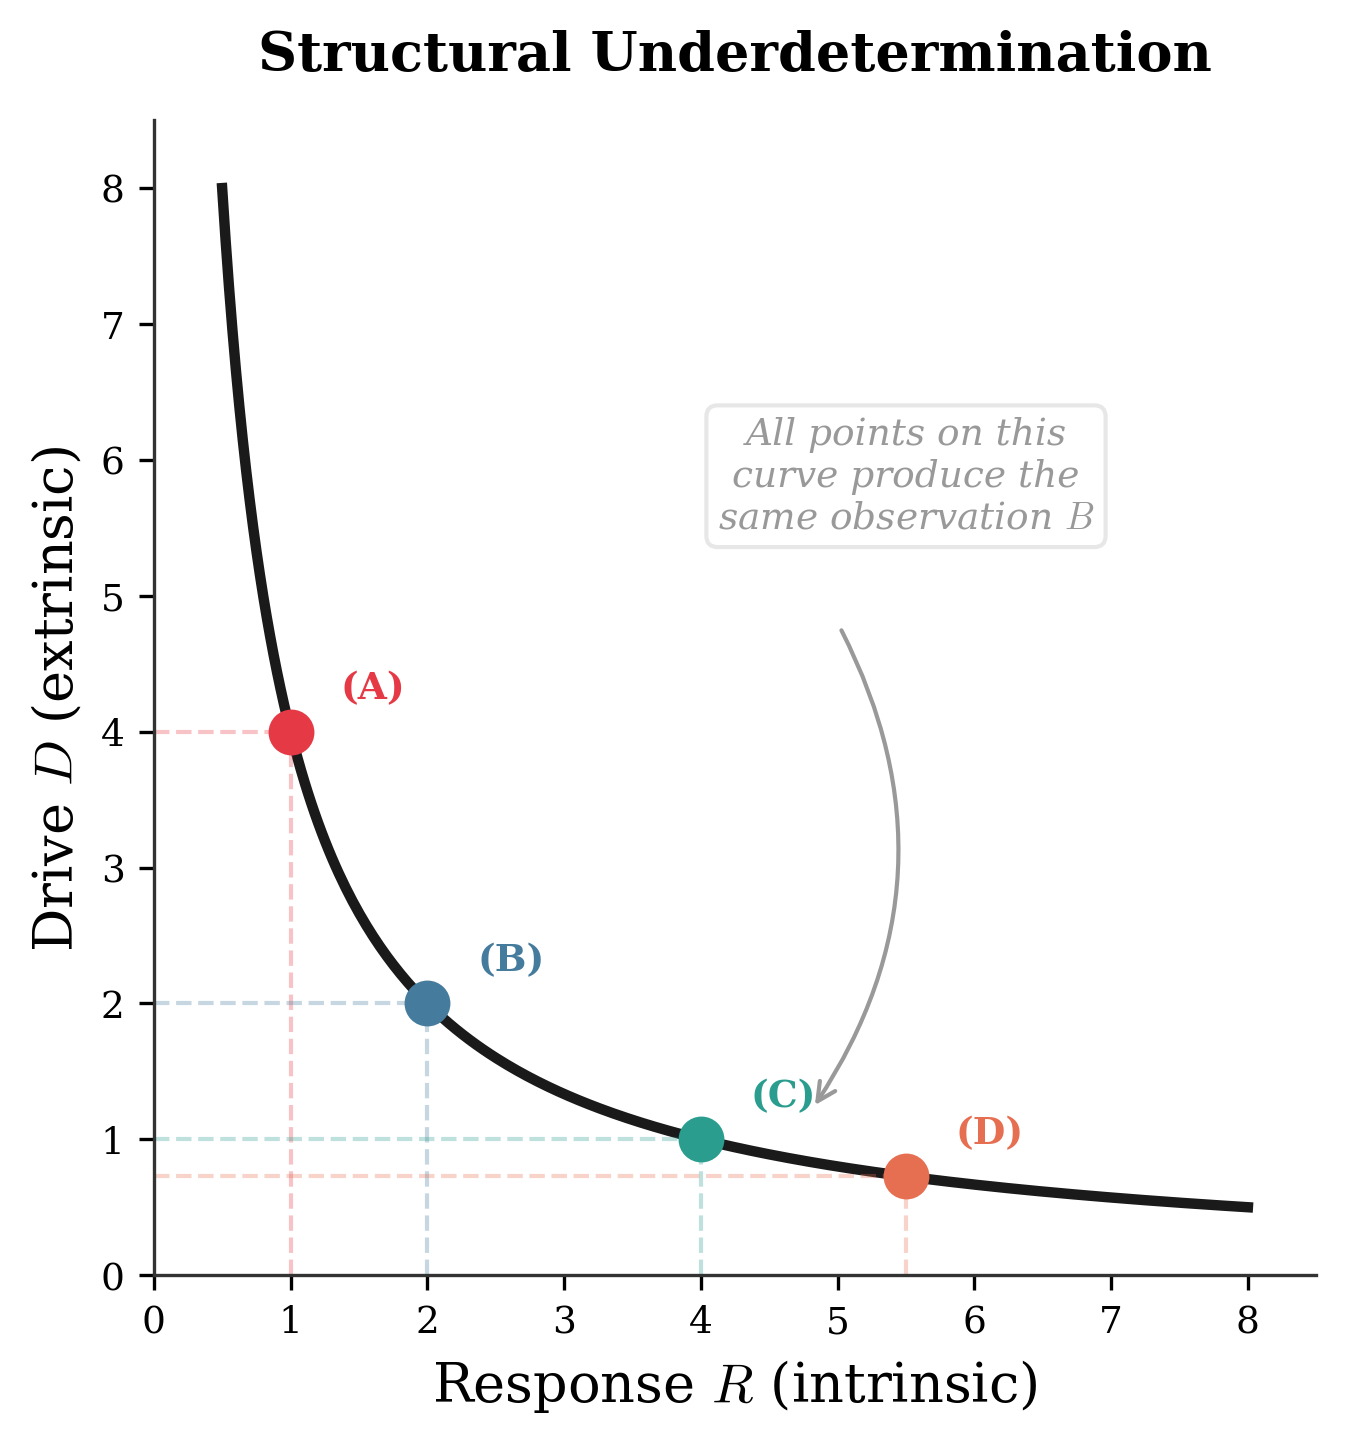
\includegraphics[width=0.55\linewidth,height=\textheight,keepaspectratio]{figures/fig_F4_underdetermination.png}

}

\caption{\label{fig-underdetermination}Structural underdetermination.
All points on the hyperbola \(B = R \times D = \text{const.}\) produce
the same observation \(B\). Different combinations of intrinsic response
\(R\) and extrinsic drive \(D\) are indistinguishable from the output
alone.}

\end{figure}%

\subsection{Physical Manifestations Across
Domains}\label{physical-manifestations-across-domains}

Part VII's five domains each instantiate this underdetermination:

\begin{longtable}[]{@{}
  >{\raggedright\arraybackslash}p{(\linewidth - 4\tabcolsep) * \real{0.3333}}
  >{\raggedright\arraybackslash}p{(\linewidth - 4\tabcolsep) * \real{0.3333}}
  >{\raggedright\arraybackslash}p{(\linewidth - 4\tabcolsep) * \real{0.3333}}@{}}
\toprule\noalign{}
\begin{minipage}[b]{\linewidth}\raggedright
Domain
\end{minipage} & \begin{minipage}[b]{\linewidth}\raggedright
Observation
\end{minipage} & \begin{minipage}[b]{\linewidth}\raggedright
Indistinguishable Alternatives
\end{minipage} \\
\midrule\noalign{}
\endhead
\bottomrule\noalign{}
\endlastfoot
Heat & Temperature history \(T(x,t)\) & High \(k\) with weak source
vs.~low \(k\) with strong source \\
Diffusion & Concentration field \(c(x,t)\) & Large \(D\) with weak
source vs.~small \(D\) with strong source \\
Electricity & Current density \(\mathbf{J}\) & High \(\sigma\) with weak
\(\mathbf{E}\) vs.~low \(\sigma\) with strong \(\mathbf{E}\) \\
Elasticity & Displacement \(\mathbf{u}(x,t)\) & Stiff material with weak
load vs.~compliant material with strong load \\
Fluids & Velocity field \(\mathbf{v}(x,t)\) & High \(\mu\) with weak
pressure gradient vs.~low \(\mu\) with strong gradient \\
\end{longtable}

In every case, the measured field is a joint consequence of intrinsic
material properties and extrinsic driving conditions. Passive
observation --- no matter how precise or prolonged --- cannot resolve
the individual contributions.

\subsection{Resolving the Ambiguity: Experimental
Calibration}\label{resolving-the-ambiguity-experimental-calibration}

To break the symmetry, one must introduce auxiliary information beyond
the observed behavior. The system identification community has long
understood this operator-level non-uniqueness (Ljung 1999); what the
present framework contributes is a formal, cross-domain statement of the
same result, grounded in the product structure common to every physical
domain.

\begin{enumerate}
\def\labelenumi{\arabic{enumi}.}
\item
  \textbf{Control the drive.} Apply a known, calibrated gradient and
  measure the response. In heat conduction: impose a measured
  temperature difference across a slab and record the steady-state heat
  flux to extract \(k\). In electricity: apply a known voltage across a
  sample and measure the current to extract \(R\). The controlled
  experiment is, at root, a method for supplying the missing equation.
\item
  \textbf{Vary one factor while holding the other fixed.} Expose the
  same material to different drives (or the same drive to different
  materials). The range of behaviors under controlled variation traces
  out the constitutive relation directly --- the very relationship that
  passive observation cannot access.
\item
  \textbf{Independent measurement.} Measure the response coefficient
  through a channel that does not involve observing the output of
  interest. In elasticity: ultrasonic wave-speed measurements extract
  the elastic moduli \(E\) and \(\nu\) without a mechanical loading
  test. In heat conduction: laser-flash diffusivity measurements excite
  and observe transient thermal response under controlled geometry.
\end{enumerate}

This is the logic of material characterization --- and, more broadly,
the logic of any experiment that seeks to separate causes from their
joint effect.

\subsection{From Physics to
Epistemology}\label{from-physics-to-epistemology}

Part I introduced the nature-nurture parallel through Lewin's equation,
\(B = f(P, E)\), where observed behavior reflects the joint action of
person and environment. With the mathematical framework now in place,
the parallel sharpens from analogy to structural identity. The
underdetermination is not merely \emph{similar} across domains --- it
arises from the same product structure.

Any system whose output is generated by the interaction of an intrinsic
factor and an extrinsic factor inherits this epistemic barrier. This
formal result has direct lineage in the Quine-Duhem thesis (Duhem 1906;
Quine 1951), which argues that empirical evidence cannot uniquely
determine the theoretical hypotheses that entail it; the present
framework makes that philosophical claim mathematically precise by
identifying the product structure as the exact source of
underdetermination. The factors differ --- conductivity versus genotype,
temperature gradient versus social environment --- but the mathematical
obstruction is the same: a single observation of the product cannot
resolve its individual factors. Twin studies and common-garden
experiments are the biologist's version of ``control the drive and vary
the response,'' and they are necessary for exactly the same structural
reason.

\subsection{Summary}\label{summary}

The product structure at the heart of this framework ---

\begin{itemize}
\tightlist
\item
  \(B = R \times D\) at the constitutive level,
\item
  \(\dot{\mathbf{z}} = \mathbf{A}_\theta \mathbf{z} + \mathbf{s}(t)\) at
  the matrix level,
\item
  \(\frac{d\mathbf{u}}{dt} = \mathbf{A}\mathbf{u} + \mathbf{S}(t)\) at
  the operator level ---
\end{itemize}

implies three conclusions:

\begin{itemize}
\tightlist
\item
  Behavior alone \textbf{cannot} resolve the intrinsic-extrinsic
  decomposition.
\item
  Controlled variation or independent measurement is \textbf{always}
  required.
\item
  Claims of ``purely intrinsic'' or ``purely extrinsic'' causation are
  \textbf{structurally unjustified} absent such controls.
\end{itemize}

This is not a limitation of measurement precision. It is a mathematical
property of interaction-structured models. The same product structure
that gives the framework its universality (one equation governing heat,
diffusion, charge, elasticity, and fluid mechanics) is what makes causal
attribution hard (one equation with two unknowns).

Parts I through IX have established the complete framework: the
structural pattern (I), energy storage and constitutive laws (II-V),
cross-domain evolution equations (VI-VII), spectral geometry of the
state manifold (VIII), and the underdetermination theorem (IX). The
framework is both general --- a single mathematical structure governs
phenomena from thermal conduction to elastic wave propagation --- and
epistemically constrained by the very interaction structure that gives
it universality.

When the extrinsic drive is no longer independent of the intrinsic
response --- whether through self-interaction, feedback, or coupling to
other dynamical systems --- the product structure itself becomes
state-dependent, and the clean factorization that underwrites both the
framework's universality and its epistemic limits requires
generalization. The underdetermination does not disappear --- it
deepens, because one can no longer cleanly define the partition one is
trying to resolve. These extensions are the subject of ongoing work.

\begin{center}\rule{0.5\linewidth}{0.5pt}\end{center}

\phantomsection\label{refs}
\begin{CSLReferences}{1}{0}
\bibitem[\citeproctext]{ref-Bird_2002}
Bird, R. Byron, Warren E. Stewart, and Edwin N. Lightfoot. 2002.
\emph{Transport Phenomena}. 2nd ed. John Wiley \& Sons.

\bibitem[\citeproctext]{ref-Brunton_2022}
Brunton, Steven L., Marko Budišić, Eurika Kaiser, and J. Nathan Kutz.
2022. {``Modern {K}oopman Theory for Dynamical Systems.''} \emph{SIAM
Review} 64 (2): 229--340. \url{https://doi.org/10.1137/21M1401243}.

\bibitem[\citeproctext]{ref-Duhem_1906}
Duhem, Pierre. 1906. \emph{La Théorie Physique: Son Objet Et Sa
Structure}. Chevalier et Rivière.

\bibitem[\citeproctext]{ref-Karnopp_2012}
Karnopp, D. C., D. L. Margolis, and R. C. Rosenberg. 2012. \emph{System
Dynamics: Modeling, Simulation, and Control of Mechatronic Systems}. 5th
ed. John Wiley \& Sons.

\bibitem[\citeproctext]{ref-Lewin_1936}
Lewin, Kurt. 1936. \emph{Principles of Topological Psychology}.
McGraw-Hill.

\bibitem[\citeproctext]{ref-Ljung_1999}
Ljung, Lennart. 1999. \emph{System Identification: Theory for the User}.
2nd ed. Prentice Hall.

\bibitem[\citeproctext]{ref-Mezic_2020}
Mezić, Igor. 2020. {``Spectrum of the {K}oopman Operator, Spectral
Expansions in Functional Spaces, and State-Space Geometry.''}
\emph{Journal of Nonlinear Science} 30: 2091--2145.
\url{https://doi.org/10.1007/s00332-019-09598-5}.

\bibitem[\citeproctext]{ref-Onsager_1931}
Onsager, Lars. 1931. {``Reciprocal Relations in Irreversible Processes.
i.''} \emph{Physical Review} 37: 405--26.
\url{https://doi.org/10.1103/PhysRev.37.405}.

\bibitem[\citeproctext]{ref-Paynter_1961}
Paynter, H. M. 1961. \emph{Analysis and Design of Engineering Systems}.
MIT Press.

\bibitem[\citeproctext]{ref-Pazy_1983}
Pazy, A. 1983. \emph{Semigroups of Linear Operators and Applications to
Partial Differential Equations}. Springer.

\bibitem[\citeproctext]{ref-Quine_1951}
Quine, Willard Van Orman. 1951. {``Two Dogmas of Empiricism.''}
\emph{The Philosophical Review} 60 (1): 20--43.
\url{https://doi.org/10.2307/2181906}.

\end{CSLReferences}




\end{document}
